\chapter{Forecasting during epidemic surges of pathogen variants capable of immune escape}
\graphicspath{{figures/ch_5/}}
\label{ch:content_3}

\section{Introduction}
\label{ch_5:sec:intro}

Accurate forecasting of epidemic surges is an important tool for public health agencies to make informed decisions about interventions and resource allocation.
Forecasting is particularly challenging when conditions in the environment change.
These changes could be due to a variety of factors including non-pharmaceutical interventions, vaccination campaigns, treatment developments, or phenotypic changes in the pathogen due to evolution.
These phenotypic changes may result in increased transmissibility, disease severity, or immune evasion, leading to surges in cases, hospitalizations, or deaths.
This has been particularly relevant throughout the COVID-19 pandemic, where the emergence of novel virus strains such as the Alpha, Delta, and Omicron variants was repeatedly accompanied by these surges.
In this work, we focus on developing forecasting methodology for these times when a new variant becomes dominant due to its ability to escape immunity induced by infections from previously circulating variants.

Forecasting epidemic surges in changing environments has previously been addressed by including time-varying parameters in infectious disease dynamics models.
These time-varying parameters can be treated as fixed inputs or estimated via parametric or non-parametric methods.
Many models focus on a time-varying transmission rate.
For example, \citet{Zhou2020Semiparametric} modeled the time-varying transmission rate via a Gaussian process.
\citet{Iyaniwura2022Mathematical} use survey data to derive separate time-varying contact rates for different subpopulations and incorporate these derived rates into their transmission rate model.
Other models include additional time-varying parameters.
In Chapter~\ref{ch:content_2}, we developed a model which included time-varying transmission rate, testing policy, and case detection rate.
In \citep{ODea2021semi}, time-varying transmission rate, reporting probability, and observation variance are modeled with random walks.
Similarly, \citet{Gibson2020real} also model time-varying transmission rate and case detection rate with random walks.
Additionally, \citet{morozova2021one} incorporate time-varying contact rate, transmission rate, recovery rate, severe fraction, hospital discharge rate, and hospital case fatality ratio into a Bayesian model.
While none of these works allow the average immune duration as varying in time, a topic of interest in this chapter, their methods could be adapted to achieve model this dynamic behavior.

Despite the apparent relevance of the novel variants, a recent comprehensive review of 136 infectious disease dynamics models noted that not one of the papers analyzed used variant prevalence data \citep{Nixon2022evaluation}.
Since that review's publication, we are aware of two papers which have attempted to use this type of data \citep{Du2023Incorporating, Rashed2022Covid}.
These two works used a deep learning framework and developed long short-term memory (LSTM) models which incorporate many data sources, including pre-processed estimates of variant proportions.

In contrast to these methods, we propose a way to integrate raw counts of variant sequences into a Bayesian compartmental model.
Rather than adapting one of the traditional models for multiple strains (see \citet{Kucharski2016Capturing} for an overview), which would necessitate many additional compartments and parameters, we propose a modification to a single strain model.
We take inspiration from \citet{Figgins2021variant}, who model variant proportions over time using a Dirichlet-multinomial likelihood to estimate variant-specific effective reproduction numbers.
Analogously, we assume that the observed count of sequences of a novel variant has a beta-binomial distribution whose mean is a product of the total number of observed genetic sequences and the proportion of the infectious population infected with the novel variant.
We then model the average duration of immunity as a flexible function of this proportion.
The form of our function ensures that the immune duration decreases when the new variant is introduced to the population, before increasing again once the new variant becomes dominant.

We evaluate our method in a simulation study wherein novel variants become dominant at varying rates and compare our forecasts to those from more conventional Bayesian compartmental models with time-varying parameters.
We demonstrate competitive or superior ability to forecast cases, hospital occupancy, ICU occupancy, and deaths, as judged by the continuous ranked probability score --- a popular proper scoring rule for probabilistic forecasts \citep{gneiting2007strictly}.
We also apply our model to real data from the Omicron wave in Orange County, California, and the state of California as a whole.
% We show superior performance of forecasting these data streams at long forecast horizons.
In particular, our proposed model is much better at forecasting the timing and size of the peak hospital occupancy, a metric crucial for public health officers making staffing decisions.


\section{Methods}
\label{ch_5:sec:methods}

\subsection{Data}
\label{ch_5:subsec:data}

We seek to integrate the following data sources into our modeling: time series of daily numbers of cases, infected hospital occupants, infected ICU occupants, deaths due to the infection, genetic sequences from a novel pathogen variant, and genetic sequences from all variants.
These time series need not be observed at the same temporal resolution, but, for clear exposition in this section, we assume they are each reported at times \( t_1, \ldots, t_L \).
We denote the vector of cases, \( \bW = \left( W_1, \ldots, W_L \right) \); infected hospital occupants, \( \bX = \left( X_1, \ldots, X_L \right) \); infected ICU occupants, \( \bY = \left( Y_1, \ldots, Y_L \right) \); deaths due to the infection, \( \bZ = \left( Z_1, \ldots, Z_L \right) \); number of genetic sequences from the novel variant, \( \bV^N =  \left( V^N_1, \ldots, V^N_L \right)\); total number of genetic sequences from all variants, \( \bV^A =  \left( V^A_1, \ldots, V^A_L \right)\). In each vector, the subscript indicates that the observation is made at the corresponding time, \( t_1, l = 1, \ldots, L \).
We work our way up to a surveillance model for these time series by first describing a transmission model for the underlying population dynamics.

\subsection{Transmission model}
\label{ch_5:subsec:transmission}

We model latent incidence and prevalence trajectories by dividing the population of interest into seven compartments: susceptible individuals \( (S) \), infected, but not yet infectious, individuals \( (E) \), infectious individuals \( (I) \), individuals hospitalized with infection \( (H) \), individuals in the ICU with infection \( (U) \),  recovered individuals \( (R) \), and individuals who died due to infection \( (D) \).
The potential progression of an individual through these states is presented in Figure~\ref{ch_5:fig:model_diagram}.
Note that we assume all deaths are transitions from the ICU compartment, not from the hospitalized or infectious compartments.
\begin{figure}
    \centering
% https://q.uiver.app/?q=WzAsNyxbMCwyLCJTIl0sWzEsMiwiRSJdLFsyLDIsIkkiXSxbNCwyLCJSIl0sWzQsMCwiRCJdLFsyLDEsIkgiXSxbMiwwLCJJQ1UiXSxbMCwxXSxbMSwyXSxbMiwzXSxbMywwLCIiLDAseyJjdXJ2ZSI6LTV9XSxbNSwzXSxbNiwzXSxbNiw0XSxbNSw2XSxbMiw1XV0=
\begin{tikzcd}[sep=scriptsize]
	&& U && D \\
	&& H \\
	S & E & I && R
	\arrow[from=3-1, to=3-2]
	\arrow[from=3-2, to=3-3]
	\arrow[from=3-3, to=3-5]
	\arrow[curve={height=-30pt}, from=3-5, to=3-1]
	\arrow[from=2-3, to=3-5]
	\arrow[from=1-3, to=3-5]
	\arrow[from=1-3, to=1-5]
	\arrow[from=2-3, to=1-3]
	\arrow[from=3-3, to=2-3]
\end{tikzcd}
    \caption[State transition diagram.]{Model diagram for potential progression between infection states.
    Model compartments are susceptible individuals \( (S) \), infected, but not yet infectious, individuals \( (E) \), infectious individuals \( (I) \), individuals hospitalized with infection \( (H) \), individuals in the ICU with infection \( (U) \),  recovered individuals \( (R) \), and individuals who died due to infection \( (D) \).}
    \label{ch_5:fig:model_diagram}
\end{figure}
We model the time-evolution of the proportions of individuals occupying these compartments with a set of ordinary differential equations (ODEs).
For simplicity, we assume a homogeneously mixing population of fixed size \( N \).
Let \( \bA(t) = \left(S(t) \right.\), \( E(t) \), \( I(t) \), \( H(t) \), \( U(t) \), \( R(t) \), \( \left. D(t) \right)^T \) denote the population proportions of all compartments at time \( t \).
We normalize \( \bA(t_0) \) so that \( \bA(t_0)^T\boldsymbol{1} = 1\), where \( \boldsymbol{1} = (1, 1, 1, 1, 1, 1, 1)^T \).
Because we fit this model to incidence data, it is convenient to also keep track of the cumulative proportion of the population that experiences transitions between compartments from \( t_0 \) to \( t \): \( \bN(t) = \left(N_{SE}(t) \right. \), \( N_{EI}(t) \), \( N_{IH}(t) \), \( N_{HU}(t) \), \( N_{UD}(t) \), \( N_{IR}(t) \), \( N_{HR}(t) \), \( N_{UR}(t) \), \( \left. N_{RS}(t) \right)^T\).
To describe mathematically how vectors $\bA(t)$ and $\bN(t)$ change through time, we first define rates of transitions between compartments, with possible transitions corresponding to the arrows in Figure~\ref{ch_5:fig:model_diagram}:

\begin{equation}
\begin{aligned}
\lambda_{SE}(S, I)  =&  \frac{\beta}{N} S I,   \\
\lambda_{EI}(E)  =& \gamma E,    \\
\lambda_{IH}(I)  =& \nu \tau I,   \\
\lambda_{HU}(H)  =& \eta  \upsilon H,   \\
\lambda_{UD}(U)  =& \omega \chi U, \\
\end{aligned}
\qquad \quad \quad
\begin{aligned}
\lambda_{IR}(I)  =& \nu \left(1 - \tau \right) I,   \\
\lambda_{HR}(H)  =& \eta \left(1 - \upsilon \right) H, \\
\lambda_{UR}(U)  =& \omega \left( 1 - \chi \right) U,    \\
\lambda_{RS}(R)  =& \kappa R,
\end{aligned}
\label{ch_5:eqn:transition_rates}
\end{equation}

where \( \beta \) is the transmission rate, \( N \) is the population size, \( 1 / \gamma  \) is the mean latent period duration, \( 1 / \nu \) is the mean infectious period duration, \( 1 / \eta \) is the mean hospitalization duration, \( 1 / \omega \) is the mean ICU stay duration, \( 1 / \kappa \) is the mean immune duration, \( \tau \) is the infection-hospitalization ratio, \( \upsilon \) is the hospitalization-ICU admission ratio, and \( \chi \) is the ICU-fatality ratio.
In some cases, we allow certain parameters to vary in time to capture changing dynamics without the needing for additional compartments in the model.
These changing dynamics could be due to policy or behavioral changes, or the presence of a new variant with increased transmissibility or immune escape.
In particular, in the models we consider in our simulation study and application, we replace \( \beta \) and \( \kappa \) with time-varying versions, \( \beta(t) \), and \( \kappa(t) \).
We discuss the details of this implementation in Section~\ref{ch_5:subsec:bayesian}.

Using the transition rates in \eqref{ch_5:eqn:transition_rates}, we define the ODEs in the model:

\begin{equation}
\begin{aligned}
\deriv{S}{t}    =&  \lambda_{RS}(R) - \lambda_{SE}(S, I), \\
\deriv{E}{t}    =&  \lambda_{SE}(S, I) - \lambda_{EI}(E),    \\
\deriv{I}{t}    =&  \lambda_{EI}(E) - \left( \lambda_{IH}(I) + \lambda_{IR}(I) \right),\\
\deriv{H}{t}    =&  \lambda_{IH}(I) - \left( \lambda_{HU}(H) +  \lambda_{HR}(H) \right),\\
\deriv{U}{t}    =&  \lambda_{HU}(H) - \left( \lambda_{UD}(U) + \lambda_{UR}(U) \right),\\
\deriv{D}{t}    =&  \lambda_{UD}(U) \\
\deriv{R}{t}    =&  \lambda_{IR}(I) + \lambda_{HR}(H) + \lambda_{UR}(U) - \lambda_{RS}(R),    \\
\end{aligned}
\qquad
\begin{aligned}
\deriv{N_{SE}}{t}  =&  \lambda_{SE}(S, I), \\
\deriv{N_{EI}}{t}  =&  \lambda_{EI}(E), \\
\deriv{N_{IH}}{t}  =&  \lambda_{IH}(I), \\
\deriv{N_{HU}}{t}  =&  \lambda_{HU}(H), \\
\deriv{N_{UD}}{t}  =&  \lambda_{UD}(U), \\
\deriv{N_{IR}}{t}  =&  \lambda_{IR}(I), \\
\deriv{N_{HR}}{t}  =&  \lambda_{HR}(H), \\
\deriv{N_{UR}}{t}  =&  \lambda_{UR}(U), \\
\deriv{N_{RS}}{t}  =&  \lambda_{RS}(R),
\end{aligned}
\label{ch_5:eqn:ODEs}
\end{equation}
subject to initial conditions \( \bA(t_0) = \left( S_0, E_0, I_0, H_0, U_0, D_0, R_0 \right) \).
Because the total population size is fixed at size \( N \), and we take \( H_0 \) , \( U_0 \), and \( D_0 \) to match the reported values of the hospitalizations, ICU occupancy, and deaths in the data at \( t_0 \), we are left with \( E_0 \), \( I_0 \), and \( R_0 \) as free parameters (because \( S_0 = N - \left( E_0 + I_0 + H_0 + U_0 + D_0 + R_0 \right) \)).
The equations in \eqref{ch_5:eqn:ODEs} are redundant, but tracking both the prevalence (left column) and the cumulative incidence (right column) is useful for linking the transmission model to data via a surveillance model.

\subsection{Surveillance model}
\label{ch_5:subsec:surveillance}

We fit the transmission model to six time series: number of new cases \( \left( \bW \right) \),  number of infected hospital occupants \( \left( \bX \right) \), number of infected ICU occupants \( \left( \bY \right) \), number of new deaths due to the infection \( \left( \bZ \right) \), number of genetic sequences from the novel variant \( \left( \bV^N \right) \), and number of genetic sequences from all variants \( \left( \bV^A \right) \) observed at time points \( t_1, \ldots t_l \).
The count for each non-genetic data stream at each time \( \left( l \right) \) is modelled by a negative binomial distribution, which we parameterize in terms of its mean \( \left( \mu \right) \) and variance \( \left( \sigma^2 \right) \).
The degree of over-dispersion in each of these negative binomial distributions is controlled by a \( \phi \) parameter.
The number of sequences from the novel variant, is modeled with a beta-binomial distribution which is conditional on the total number of observed sequences.
We parameterize this distribution in terms of \( \delta \), its mean success probability and \( \phi \), an over-dispersion parameter.

We model the observed cases, \( W_l \), in the interval \( \left( t_{l - 1}, t_l \right] \), for \( l =1 \ldots L \), by
% cases
\begin{equation}
W_l \sim \operatorname{Negative Binomial} \left( \mu^{W}_l = \rho^W \cdot N \cdot \Delta N_{EI} \left( t_l \right), \left(\sigma^W_l\right)^{2} = \mu^{W}_l \left( 1 + \mu^{W}_l / \phi_W \right) \right),
\label{ch_5:eqn:case_emission}
\end{equation}
where \( \rho^W \in [0,1]\) is the overall case detection rate, meaning that the number of observed cases is assumed to be some noisy realization of the fraction of the true new cases in the population, as estimated by the ODE model.
In some models, we allow the case detection rate to vary over time, in which case we replace \( \rho^W \) with \( \rho^W \left( t_l \right) \) in \eqref{ch_5:eqn:case_emission}.
We discuss modeling choices for this and \( \delta \left( t_l \right) \) in the next section.

The observed number of hospital occupants with an infection at time \( t_l \) is modeled by
% hospi
\begin{equation}
X_l \sim \operatorname{Negative Binomial} \left( \mu^{X}_l = N \cdot H \left( t_l \right), \left(\sigma^X_l\right)^{2} = \mu^{X}_l \left( 1 + \mu^{X}_l / \phi_X \right) \right),
\label{ch_5:eqn:hosp_emission}
\end{equation}
which means that the observed number of hospital occupants is a noisy realization of the hospitalized population, as estimated by the ODE model.

We assume that the number of ICU occupants with an infection has the distribution
% icu
\begin{equation}
Y_l \sim \operatorname{Negative Binomial} \left( \mu^{Y}_l = N \cdot U \left( t_l \right), \left(\sigma^Y_l\right)^{2} = \mu^{Y}_l \left( 1 + \mu^{Y}_l / \phi_Y \right) \right),
\label{ch_5:eqn:icu_emission}
\end{equation}
indicating that the observed number of ICU occupants is a noisy realization of the ICU population, as estimated by the ODE model.

The observed deaths due to the infection are modeled by
% deaths
\begin{equation}
Z_l \sim \operatorname{Negative Binomial} \left( \mu^{Z}_l = \rho^Z \cdot N \cdot \Delta N_{UD} \left( t_l \right), \left(\sigma^Z_l\right)^{2} = \mu^{Z}_l \left( 1 + \mu^{Z}_l / \phi_Z \right) \right),
\label{ch_5:eqn:death_emission}
\end{equation}
where \( \rho^Z \in [0,1]\) is the overall death detection rate, meaning that the number of observed deaths is assumed to be some noisy realization of the fraction of the true new deaths in the population, as estimated by the ODE model.

We model the observed counts of genetic sequences of the novel variant, conditional on the observed number of all genetic sequences by
\begin{equation}
V^N_l \sim \operatorname{Beta-Binomial} \left( V^A_l, \alpha = \phi_V \delta \left( t_l \right), \beta = \phi_V \left( 1 -  \delta \left( t_l \right) \right) \right),
\label{ch_5:eqn:novel_variant_emission}
\end{equation}
where \( \delta \left( t_l \right) \) is the proportion of currently infectious individuals who are infected with the novel variant.
Thus, the observed proportion of genetic sequences of the novel variant is a noisy realization of the true proportion in the population.

\subsection{Bayesian inference}
\label{ch_5:subsec:bayesian}

In Sections~\ref{ch_5:subsec:transmission} and \ref{ch_5:subsec:surveillance}, we noted that, for some models considered in this work, \( \beta \), \( \kappa \), and \( \rho^W \) could be substituted for time-varying counterparts, \( \beta(t) \), \( \kappa(t) \), and \( \rho^W(t) \).
We now present some options for modeling how these parameters may change over time.
We proceed by reparameterizing \( \beta(t) \) as  basic reproduction number, \( R_0(t) = \beta(t) / \nu \), and \( \kappa(t) \) as the average immune duration, \( 1 / \kappa(t) \).

In some models, we parameterize \( R_0(t) \), \( 1 / \kappa(t) \), or \( \rho^2(t) \) as piecewise constant functions, where each vector defining the constants a prior follows a Gaussian Markov random field (GMRF).
More precisely, we define the auxiliary vectors:
\begin{gather*}
\brtilde = (\tilde{R}_{0,1}, \tilde{R}_{0,2}, \ldots, \tilde{R}_{0,L}) \text{, }
\bkappatilde = (\kappatilde_1, \kappatilde_2, \ldots, \kappatilde_L)  \text{, and }
\brhowtilde = (\brhowtilde_1, \brhowtilde_2, \ldots, \brhowtilde_L),
\end{gather*}
which follow the Gaussian Markov random field priors
\begin{equation}
\begin{aligned}
	\tilde{R}_{0,l} \sim& N\left(\tilde{R}_{0, l - 1}, \sigma_{R_0}^2\right)\text{, where } l=2,\ldots,L \text{ and } \tilde{R}_{0,1} \sim N\left(\mu_{R_{01}},\sigma^2_{R_{01}}\right),\\
	\frac{1}{\kappatilde_{l}} \sim& N\left(\frac{1}{\kappatilde_{l - 1}}, \sigma_\kappa^2\right)\text{, where } l=2,\ldots,L \text{ and } \frac{1}{\kappatilde_1} \sim N\left(\mu_{\kappa_1},\sigma^2_{\kappa_1}\right),\\
	\rhowtilde_{l} \sim& N\left(\rhowtilde_{l - 1}, \sigma_{\rho^Y}^2\right)\text{, where } l=2,\ldots,L \text{ and } \rhowtilde_1 \sim N\left(\mu_{\rho^Y_1}, \sigma^2_{\rho^Y_1}\right),
 \label{ch_5:eqn:GMRF}
\end{aligned}
\end{equation}
and define the piecewise constant functions:
\begin{align}
	R_0(t) =& \sum_{l=1}^L \exp{\left( \tilde{R}_{0,l} \right) \1{t \in (t_{l-1}, t_l]}},\\
	1 / \kappa(t) =& \sum_{l=1}^L \exp{\left( 1 / \kappatilde_l \right)\ \1{t \in (t_{l-1}, t_l]} },\\
	\rho^W(t) =& \sum_{l=1}^L \frac{\exp{\left( \rhowtilde_l \right) \1{t \in (t_{l-1}, t_l]} }}{\exp{\left( \rhowtilde_l \right) \1{t \in (t_{l-1}, t_l]} } + 1}.
\end{align}

In our simulation study and application, we assume that these time-varying dynamics are due to the emergence of a novel variant to which the population has reduced immunity.
Thus, we hypothesize that defining time-varying parameters as a function of \( \delta(t) \), the proportion of currently infectious individuals who are infected with the novel variant, may lead to improvements in forecasting capabilities.
In principle, we can do this for any of the parameters in the model that might differ by variant, but we only consider this parameterization for the average immune duration, \( 1 / \kappa \), in our simulation study and application.
We model \( 1 / \kappa(t) \) as dependent on \( \delta(t) \) by
\begin{equation}
    1 / \kappa(t) = 1 / \hat{\kappa}\left( \delta (t + \zeta) \right) = \exp \left\{ \alpha_0 + \alpha_1 \left[ \delta(t + \zeta) \left( 1 - \delta(t + \zeta) \right) \right]^{\alpha_2} \right\},
    \label{ch_5:eqn:kappa_delta}
\end{equation}
where \( \alpha_2 > 0 \).
This functional form ensures that the average immune duration is maximized when the entire infectious population is infected with the same variant (i.e., \( \delta = 0 \) or \( \delta = 1 \)) and minimized when \( \delta = 0.5 \).
Thus, when a new variant is introduced, but only constitutes a small proportion of the infectious population, the average immune duration begins to decrease, moving more of the population to the susceptible compartments.
The immune duration continues to decrease until the new variant is half of the infectious population, at which point there is a large infectious population carrying the new variant and a large proportion of the population with reduced immunity to the new variant.
As the new variant reaches dominance, the immune duration returns to its original level.
We allow this relationship to be flexible by including an offset in time, \( \zeta \).

We note that the maximum immune duration is \( \exp \left( \alpha_0 \right)\), and the minimum immune duration is \(\exp \left\{ \alpha_0 + \alpha_1 \left( 1/4  \right)^{\alpha_2} \right\} \).
To use a more interpretable prior, we reparameterize \( \alpha_1 \) in terms of \( \alpha_1^* \):
\begin{equation}
    \alpha_1 = 4^{\alpha_2} \ln \left( \alpha_1^* \right).
    \label{ch_5:eqn:alpha_1}
\end{equation}
Then the minimum immune duration is 
\( \exp \left\{ \alpha_0 + 4^{\alpha_2} \ln \left( \alpha_1^* \right) \left( 1/4  \right)^{\alpha_2} \right\} = \alpha_1^* \exp \left\{ \alpha_0 \right\} \).
Recalling that \( \exp \left\{ \alpha_0 \right\} \) is the maximum immune duration, we see that  \( \alpha_1^* \in [0,1] \) is simply a scaling factor, which determines the minimum duration, based on the maximum duration.
We show several example curves for \eqref{ch_5:eqn:kappa_delta} in Figure~\ref{ch_5:fig:example_immune_durration_plot}.

\begin{figure}
    \centering
    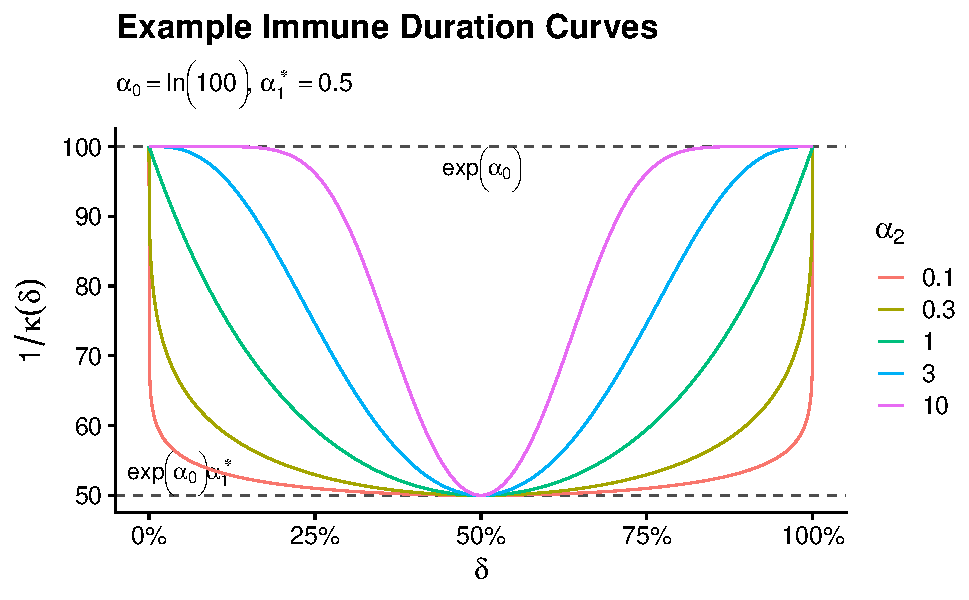
\includegraphics[width=1.0\columnwidth]{example_immune_durration_plot.pdf}
    \caption[Example immune duration curves.]{Example immune duration curves for several values of \( \alpha_2 \), with \( \alpha_0 = \ln\left(100\right), \alpha_1^* = 0.5 \).
    The full formula for these curves is given by \eqref{ch_5:eqn:kappa_delta} and \eqref{ch_5:eqn:alpha_1}.}
    \label{ch_5:fig:example_immune_durration_plot}
\end{figure}

Now, we discuss our model for \( \delta(t) \), the proportion of currently infectious individuals who are infected with the novel variant.
We assume that, after the novel variant is introduced, its proportion in the population evolves according to logistic growth:
\begin{equation}
    \delta(t) = \frac{\exp \left\{ \iota_0 + \iota_1 \left( t \right) \right\}}{\exp \left\{ \iota_0 + \iota_1 \left( t \right) \right\} + 1}.
    \label{ch_5:eqn:logistic_growth}
\end{equation}
This parametric approach is borrowed from population genetics literature devoted to studying the dynamics of the novel variant proportion in the population of interest \citep{Lacerda2014Population, Zhao2023mechanism}.
To set interpretable priors on \( \iota_0 \) and \( \iota_1 \), we parameterize the logistic growth as 
\begin{equation}
    \delta(t) = \frac{\exp \left\{ \iota_0 + \iota_1 \left( t - t^* \right) \right\}}{\exp \left\{ \iota_0 + \iota_1 \left( t - t^* \right) \right\} + 1},
\end{equation}
where \( t^* \) is the time point for which \( \delta(t^*) = \frac{ \exp \left\{ \iota_0 \right\} }{\exp \left\{ \iota_0 \right\} + 1} \).
Then \( \iota_1 = \frac{\ln \left( \frac{0.99}{1 - 0.99} \right) - \ln \left( \frac{0.01}{1 - 0.01} \right)}{\iota_1^*} \), where \( \iota_1^* \) is the amount of time the novel variant takes to grow from 1\% of the infectious population to 99\% of the infectious population.

With these parameters all defined, we describe our Bayesian procedure.
We collect all our model parameters into a vector $\boldsymbol{\theta}$ and write the likelihood function as 
\begin{align*}
& \Pr\left(\bW, \bX, \bY, \bZ, \bV^N \mid \btheta \right) \\
=& \Pr\left(\bW \mid \btheta \right) \Pr\left(\bX \mid \btheta \right) \Pr\left(\bY \mid \btheta \right) \Pr\left(\bZ \mid \btheta \right) \Pr\left(\bV^N \mid \btheta \right)    \\
=&   \prod_{l=1}^{L} \Pr\left(W_l \mid \btheta \right) \Pr\left(X_l \mid \btheta \right) \Pr\left(Y_l \mid \btheta \right) \Pr\left(Z_l \mid \btheta \right) \Pr\left(V^N_l \mid \btheta \right) ,
\end{align*}
where \( \Pr\left(W_l \mid \btheta \right) \), \( \Pr\left(X_l \mid \btheta \right) \), \( \Pr\left(Y_l \mid \btheta \right) \), \( \Pr\left(Z_l \mid \btheta \right) \), and \( \Pr\left(V^N_l \mid \btheta \right) \), are the probability mass functions given by \eqref{ch_5:eqn:case_emission}, \eqref{ch_5:eqn:hosp_emission}, \eqref{ch_5:eqn:icu_emission}, \eqref{ch_5:eqn:death_emission}, and \eqref{ch_5:eqn:novel_variant_emission}, respectively.
We encode available information about our model parameters in a prior distribution with density $\pi(\btheta)$.
We assume that all univariate non-GMRF distributed parameters are \textit{a priori} independent and list our prior assumptions for our simulation study in Table~tk and for our application in Table~tk.
We base all our inferences and predictions on the posterior distribution of all model parameters:
\begin{equation}
\Pr\left(\btheta \mid \bW, \bX, \bY, \bZ, \bV^N \right) \propto \Pr\left(\bW, \bX, \bY, \bZ, \bV^N \mid \btheta \right) \pi \left( \btheta \right).
\end{equation}
We sample from this posterior using the No-U-Turn Sampler, \citep{NUTS} as implemented in the Turing Julia package \citep{turing}.
Model code and data are available at the following GitHub repository: \url{https://github.com/damonbayer/immunity_semi_parametric_model}.

In total, the form of the model without any GMRF components has 24 parameters.
Adding a GMRF component requires one additional parameter for the variance and one more parameter per observation time.
In our simulation study and real data analyses, the number of model parameters ranges between 24 and 91.

\section{Results}
\label{ch_5:sec:results}

\subsection{Simulation study}
\label{ch_5:subsec:simulation}

We simulate three data sets for this study, each where the novel variant becomes dominant at a different speed: slow (24 weeks to go from 1\% to 99\% of sequences), medium (13 weeks), and fast (7 weeks).
The data sets are simulated from a two strain model, which is depicted in Figure~\ref{ch_5:fig:full_model_diagram_compact} and explained in full detail in Appendix~\ref{ch_5:sec:full_simulation_model_explanation}.
Briefly, the model is similar to the one depicted in Figure~\ref{ch_5:fig:model_diagram} but is modified to account for two distinct disease variants.
The variants associated with each compartment are indicated by the subscripts: ``N" for the novel variant, ``O" for other variants, and ``A" for all types for variants.
When all compartments associated with one variant type are empty, the model is equivalent to the one from Figure~\ref{ch_5:fig:model_diagram}.

These otherwise independent models are linked by allowing transitions from \( S_A \) and \( R_O \) to \( E_N \).
That is, people who are susceptible to all variant types (\( S_A \)) and those who are only recovered from other variants (\( R_O \)) can become infected with the novel variant (\( E_N \)).
The rates for these transitions are given by
\begin{equation}
   \lambda_{{S_A}{E_N}}\left( S_A, I_N \right) = \frac{\beta}{N} S_A I_N \quad \textrm{and} \quad \lambda_{{R_O}{E_N}}\left( R_O, I_N \right) = \epsilon \frac{\beta}{N} R_O I_N,
\end{equation}
where \( \beta \) and \( N \) are defined as in \eqref{ch_5:eqn:transition_rates}, and \( \epsilon \in [0, 1] \) is a factor that represents the effect of partial immunity to the novel variant conferred by a recent infection from  another variant.
After some time, all the individuals in the \( O \) subscript compartments will have transitioned to the \( N \) subscript compartments, and the model again behaves like the one in Figure~\ref{ch_5:fig:model_diagram}.

\begin{table}
\caption{Simulation parameters that differ by scenario.}
\label{ch_5:table:scenario_differing_parameters}
\centering
\label{table}
\begin{tabular}{lrr}
Scenario & \( \beta \) & \( \epsilon \) \\ \hline
Slow     & 2.1         & 0.75           \\
Medium   & 2.1         & 1.0            \\
Fast     & 3.5         & 1.0            \\
\end{tabular}
\end{table}

\begin{figure}
    \centering
% https://q.uiver.app/?q=WzAsMTMsWzAsMCwiU18wIl0sWzEsMCwiRV8xIl0sWzIsMCwiSV8xIl0sWzIsMSwiUl8xIl0sWzEsMiwiRV97Mn0iXSxbMiwyLCJJXzIiXSxbMiwzLCJSXzIiXSxbMCwyLCJTXzIiXSxbMywwLCJIXzEiXSxbNCwwLCJJQ1VfMSJdLFszLDIsIkhfMiJdLFs0LDIsIklDVV8yIl0sWzQsMSwiRCJdLFswLDFdLFsxLDJdLFsyLDNdLFswLDRdLFs0LDVdLFszLDBdLFszLDRdLFs1LDZdLFs2LDddLFsyLDhdLFs4LDldLFs5LDNdLFs4LDNdLFs1LDEwXSxbMTAsNl0sWzEwLDExXSxbMTEsNl0sWzcsNF0sWzExLDEyXSxbOSwxMl1d
\begin{tikzcd}[sep=scriptsize]
	% {S_0} & {E_1} & {I_1} & {H_1} & {U_1} \\
	% && {R_1} && D \\
	% {S_2} & {E_2} & {I_2} & {H_2} & {U_2} \\
	% && {R_2}
        {S_A} & {E_O} & {I_O} & {H_O} & {U_O} \\
	&& {R_O} && {D_A} \\
	{S_N} & {E_N} & {I_N} & {H_N} & {U_N} \\
	&& {R_N}
	\arrow[from=1-1, to=1-2]
	\arrow[from=1-2, to=1-3]
	\arrow[from=1-3, to=2-3]
	\arrow[from=1-1, to=3-2]
	\arrow[from=3-2, to=3-3]
	\arrow[from=2-3, to=1-1]
	\arrow[from=2-3, to=3-2]
	\arrow[from=3-3, to=4-3]
	\arrow[from=4-3, to=3-1]
	\arrow[from=1-3, to=1-4]
	\arrow[from=1-4, to=1-5]
	\arrow[from=1-5, to=2-3]
	\arrow[from=1-4, to=2-3]
	\arrow[from=3-3, to=3-4]
	\arrow[from=3-4, to=4-3]
	\arrow[from=3-4, to=3-5]
	\arrow[from=3-5, to=4-3]
	\arrow[from=3-1, to=3-2]
	\arrow[from=3-5, to=2-5]
	\arrow[from=1-5, to=2-5]
\end{tikzcd}
    \caption[Compartmental diagram for simulation model.]{Compartmental diagram for simulation model.
    Model compartments are susceptible individuals \( (S) \), infected, but not yet infectious, individuals \( (E) \), infectious individuals \( (I) \), individuals hospitalized with infection \( (H) \), individuals in the ICU with infection \( (U) \),  recovered individuals \( (R) \), and individuals who died due to infection \( (D) \).
    The variants associated with each compartment are indicated by the subscripts: ``N" for the novel variant, ``O" for other variants, and ``A" for all types for variants.}
    \label{ch_5:fig:full_model_diagram_compact}
\end{figure}

For our simulations, the compartments are initiated with the entire population (3 million) in \( S_0 \), except a small number who are in \( E_O \).
Because all the \( N \) subscript compartments are empty, this behaves like the model in Figure~\ref{ch_5:fig:model_diagram}.
We simulate the compartment trajectories until the initial surge begins to subside.
While the overall prevalence is beginning to decrease, we simulate an importation of 1000 people who are infectious with the novel variant into the \( I_N \) compartment.
Then, the individuals begin to transition into the \( N \) subscript compartments, resulting in a second wave.
Forecasting this second wave is the objective of our modeling efforts.

We manipulate the size of this wave and the speed with which the novel variant takes over by altering \( \beta \) and \( \epsilon \) in the different simulation settings.
Table~\ref{ch_5:table:scenario_differing_parameters} presents the  the exact \( \beta \) and \( \epsilon \) values used.
The other simulation parameters are given in Table~tk.
Changes of the resulting proportion of individuals infected with the novel variant over time for each simulated scenario is presented in Figure~\ref{ch_5:fig:proportion_novel_variant_simulated_data_plot}.
The simulated data for the medium takeover speed scenario is plotted in Figure~\ref{ch_5:fig:simulated_binned_data_medium_plot}, with the gray shaded areas indicating the time points for which we produce forecasts.
Similar figures for the other data sets are presented in Figures~\ref{ch_5:fig:simulated_binned_data_slow_plot} and \ref{ch_5:fig:simulated_binned_data_fast_plot}.
In each scenario, non-genetic data is reported at a weekly resolution, starting 20 weeks into the simulation, which we call \( t = 0 \).
Genetic data is reported at a daily resolution, which is crucial to capturing the early exponential-like growth of the novel variant, relative to the other variants.
Additionally, the genetic data is only reported beginning one week before the novel variant import event, which is necessary to meet the assumption of logistic growth in \eqref{ch_5:eqn:logistic_growth}.

\begin{figure}
    \centering
    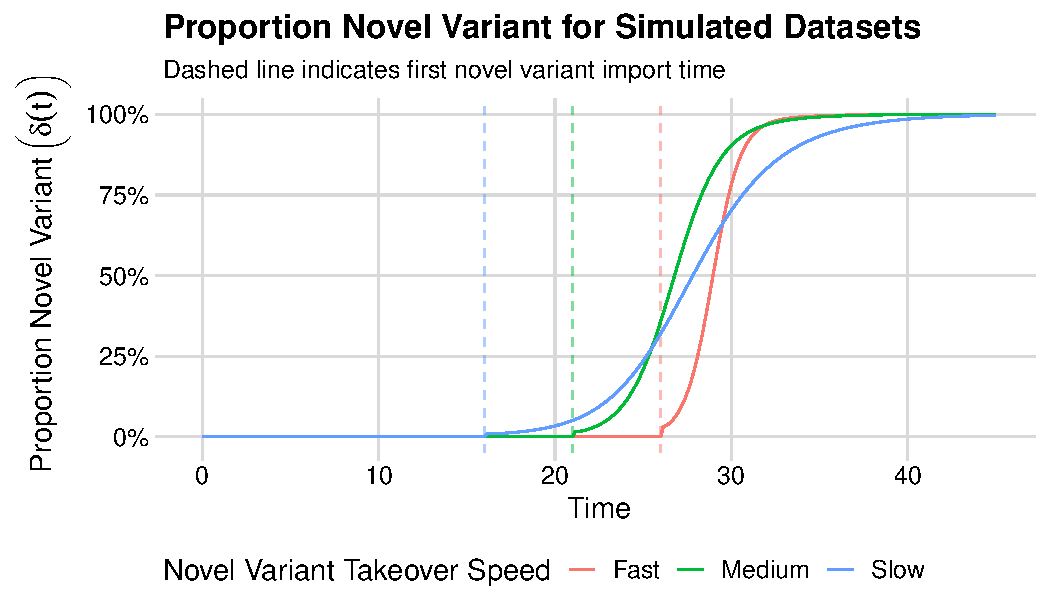
\includegraphics[width=1.0\columnwidth]{proportion_novel_variant_simulated_data_plot}
    \caption{Proportion of infectious individuals infected with the novel variant over time for three simulated scenarios.
    The dashed line indicates the time that the initial importation event of the novel variant occurs.}
    \label{ch_5:fig:proportion_novel_variant_simulated_data_plot}
\end{figure}

\begin{figure}
    \centering
    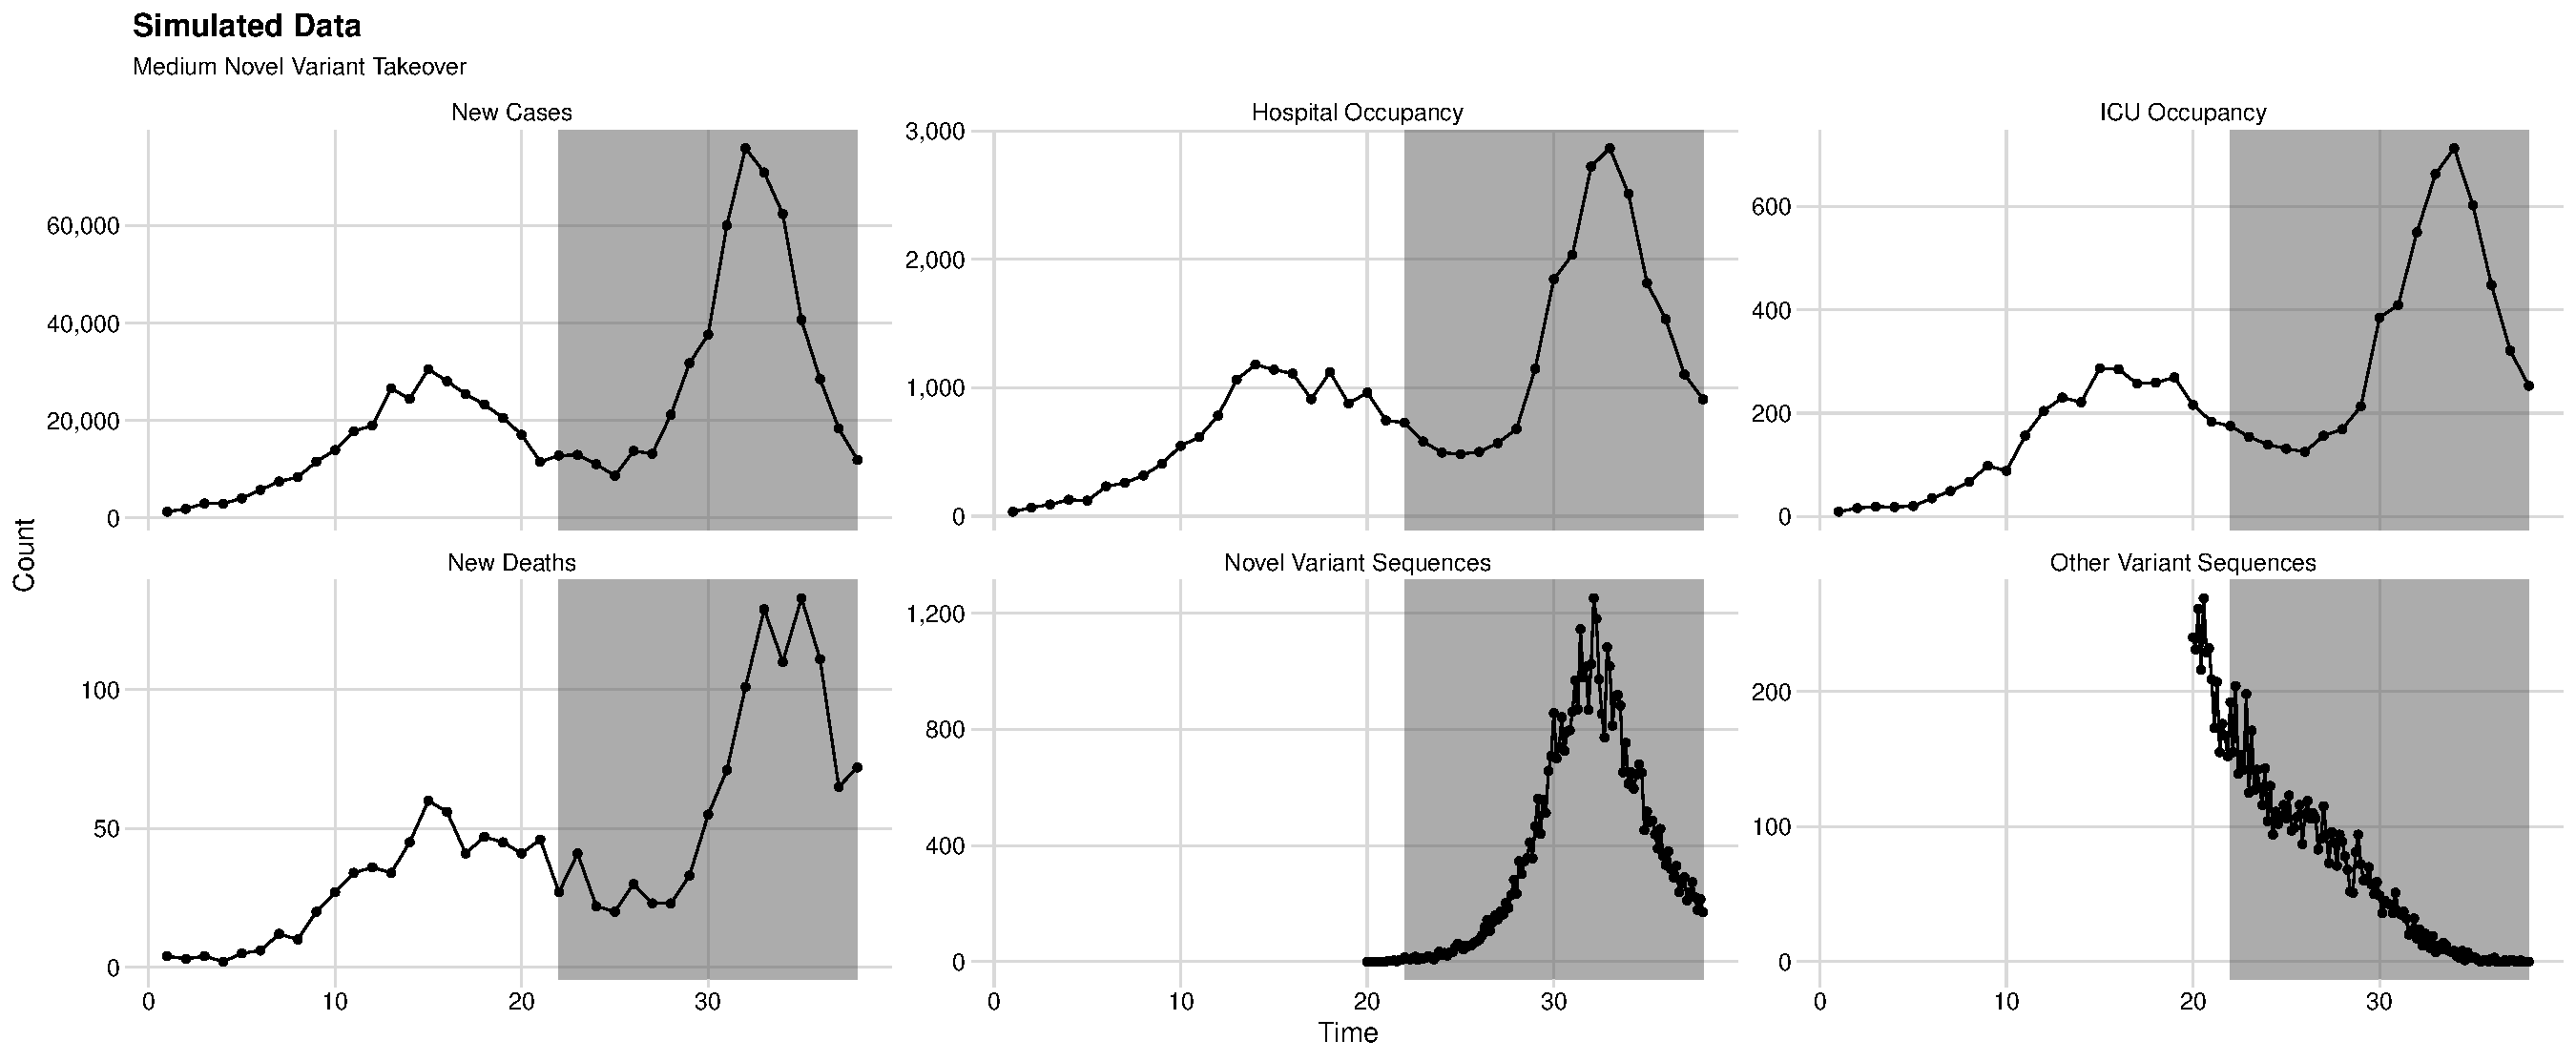
\includegraphics[width=1.0\columnwidth]{simulated_binned_data_medium_plot}
    \caption[Simulated data set for the medium takeover speed scenario.]{Simulated data set for the medium takeover speed scenario.
    The gray shaded areas indicate the time points for which we produce forecasts}
    \label{ch_5:fig:simulated_binned_data_medium_plot}
\end{figure}

We fit three models to these simulated data sets: (1) a model where \( R_0(t) \) is a priori modeled as a GMRF and \( 1 / \kappa(t) \) is constant, (2) a model where \( R_0(t) \) is constant and \( 1 / \kappa(t) \) is a priori modeled as a GMRF, and (3) a model where \( R_0(t) \) is constant and \( 1 / \kappa(t) \) is a function of the proportion of infectious individuals infected with the novel variant shown in \eqref{ch_5:eqn:kappa_delta}.
The first model is reflective of typical practice in infectious disease modeling (see, e.g., \citep{Gibson2020real, ODea2021semi}).
The second is a slight variation on the first, where we make the immunity duration, rather than the basic reproductive number, vary over time.
The third model is our main innovation, which models the mean immune duration based on genetic data.
The priors used in these models are presented in Table~tk.
For each simulated data set, we used four Markov chains run in parallel to draw a total of 1000 posterior samples.

While these models forecast several data streams, we present only forecasts related to hospitalization in the main text, as they are the most relevant for public health policymakers.
We present additional results for cases, ICU occupancy, and deaths in Section~\ref{ch_5:sec:sim_cases_icu_death}.
In general, these results exhibit the same patterns as observed in the hospitalization results.
Additionally, we conducted a sensitivity analysis wherein we modified the prior for the anticipated speed of the novel variant takeover and found our model to be robust to these changes.
The results of this analysis are presented in Section~\ref{ch_5:sec:sim_sensitivity}.

We first show 1, 2, and 4-week ahead forecasts for the simulated medium takeover speed data in Figure~\ref{ch_5:fig:simulated_forecast_comparison_data_hospitalizations_medium_plot}.
Analogous plots for the slow and fast takeover data are presented in Figures~\ref{ch_5:fig:simulated_forecast_comparison_data_hospitalizations_slow_plot} and \ref{ch_5:fig:simulated_forecast_comparison_data_hospitalizations_fast_plot}, respectively.

From these figures, we note that, for all models and all data sets, one-week ahead forecasts match the data quite closely.
As may be expected, performance degrades as the forecast horizon increases.
For the slow takeover data, the forecasts where \( 1 / \kappa(t) \) is informed by the genetic data closely match the data up to the four-week ahead forecasts.
The forecasts where \( 1 / \kappa(t) \) is a priori modeled as a GMRF also match the data quite well, while the model where \( R_0(t) \) is a priori modeled as a GMRF is much less sharp than the other models.
For the medium data, the forecasts with \( 1 / \kappa(t) \) informed by the genetic data again predict the data well up to the four-week forecast horizon.
The \( 1 / \kappa(t) \) GMRF model misjudges the height and the timing of the peak, and the forecasts from the \( R_0(t) \) GMRF model are again much wider than the other models.
When forecasting the fast variant takeover data, the \( R_0(t) \) GMRF model is competitive with the \( 1 / \kappa(t) \) genetic model, while the \( 1 / \kappa(t) \) GMRF model again misjudges the peak.

\begin{figure}
    \centering
    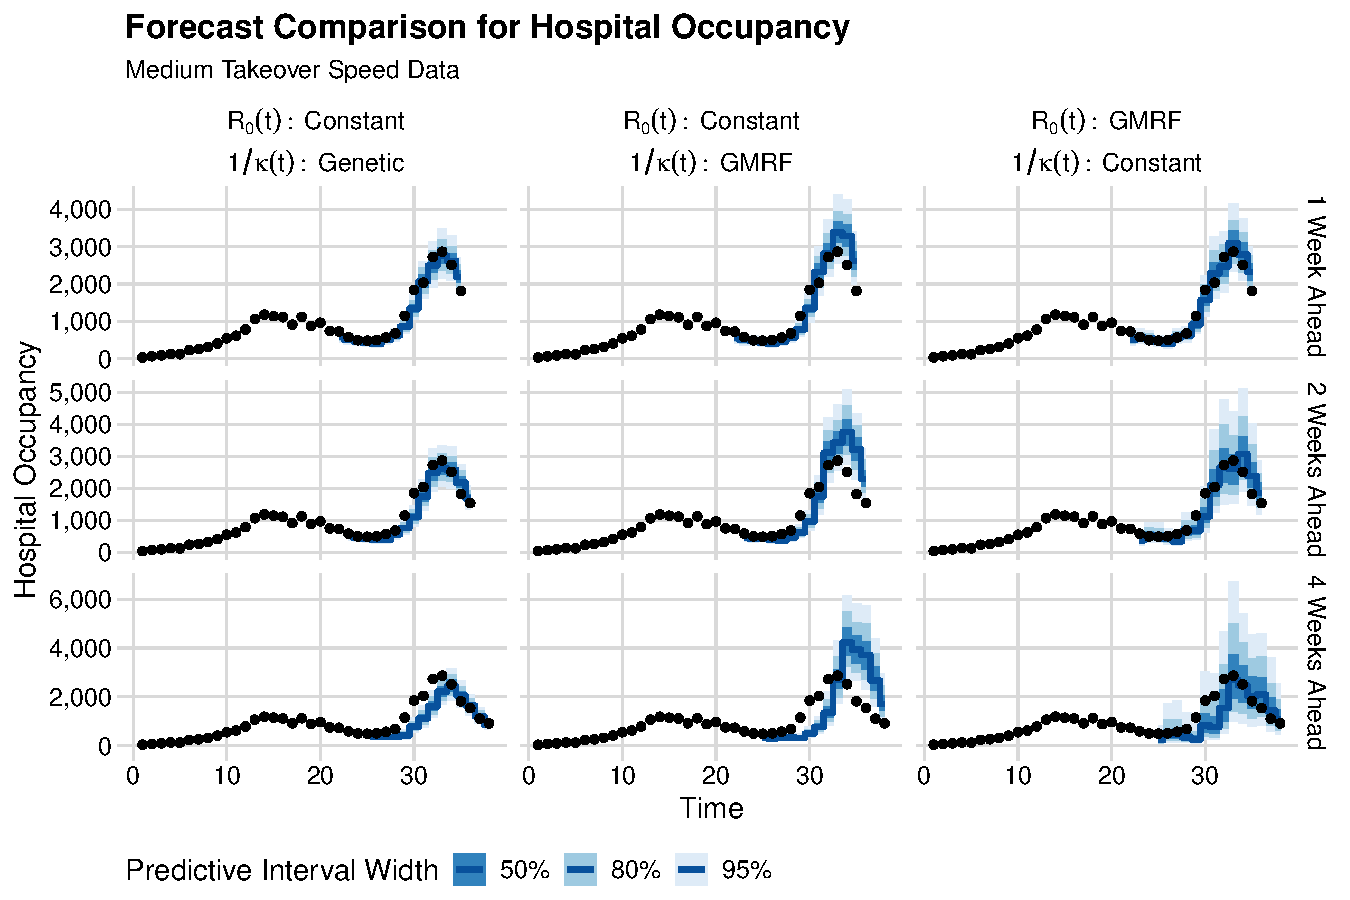
\includegraphics[width=1.0\columnwidth]{simulated_forecast_comparison_data_hospitalizations_medium_plot}
    \caption[Hospital occupancy forecasts for simulated medium takeover speed data.]{Hospital occupancy forecasts from three models at 1, 2, and 4-week forecast horizons for the simulated medium takeover speed data.}
    \label{ch_5:fig:simulated_forecast_comparison_data_hospitalizations_medium_plot}
\end{figure}

To numerically assess the quality of these forecasts, we compute the continuous ranked probability score (CRPS) for each forecast at 1, 2, and 4-week horizons.
Plots summarizing the average scores of the hospitalization forecasts are displayed in Figure~\ref{ch_5:fig:simulated_crps_comparison_dotplot_data_hospitalizations_plot}.
Analogous plots for forecasts of cases, ICU occupancy, and deaths are presented in Figures~\ref{ch_5:fig:simulated_crps_comparison_dotplot_data_new_cases_plot}--\ref{ch_5:fig:simulated_crps_comparison_dotplot_data_new_deaths_plot}.
Additionally, we show the scores for each individual forecast for each data stream in Figures~\ref{ch_5:fig:simulated_crps_comparison_data_new_cases_plot}--\ref{ch_5:fig:simulated_crps_comparison_data_new_deaths_plot}.
We observe that for the slow and medium takeover speed scenarios, the model where \( 1 / \kappa(t) \) is informed by the genetic data achieves the lowest (best) average scores.
For the slow takeover data, the model where \( 1 / \kappa(t) \) is modeled by a GMRF performs better than the model where \( R_0(t) \) is a priori modeled as a GMRF.
For the medium takeover data, the two GMRF models are more competitive with each other.
With respect to the fast takeover scenario, the model where \( R_0(t) \) is modeled as a GMRF achieves slightly lower scores than the model that uses genetic data, and both of these models outperform the model where  \( 1 / \kappa(t) \) is modeled as a GMRF.

\begin{figure}
    \centering
    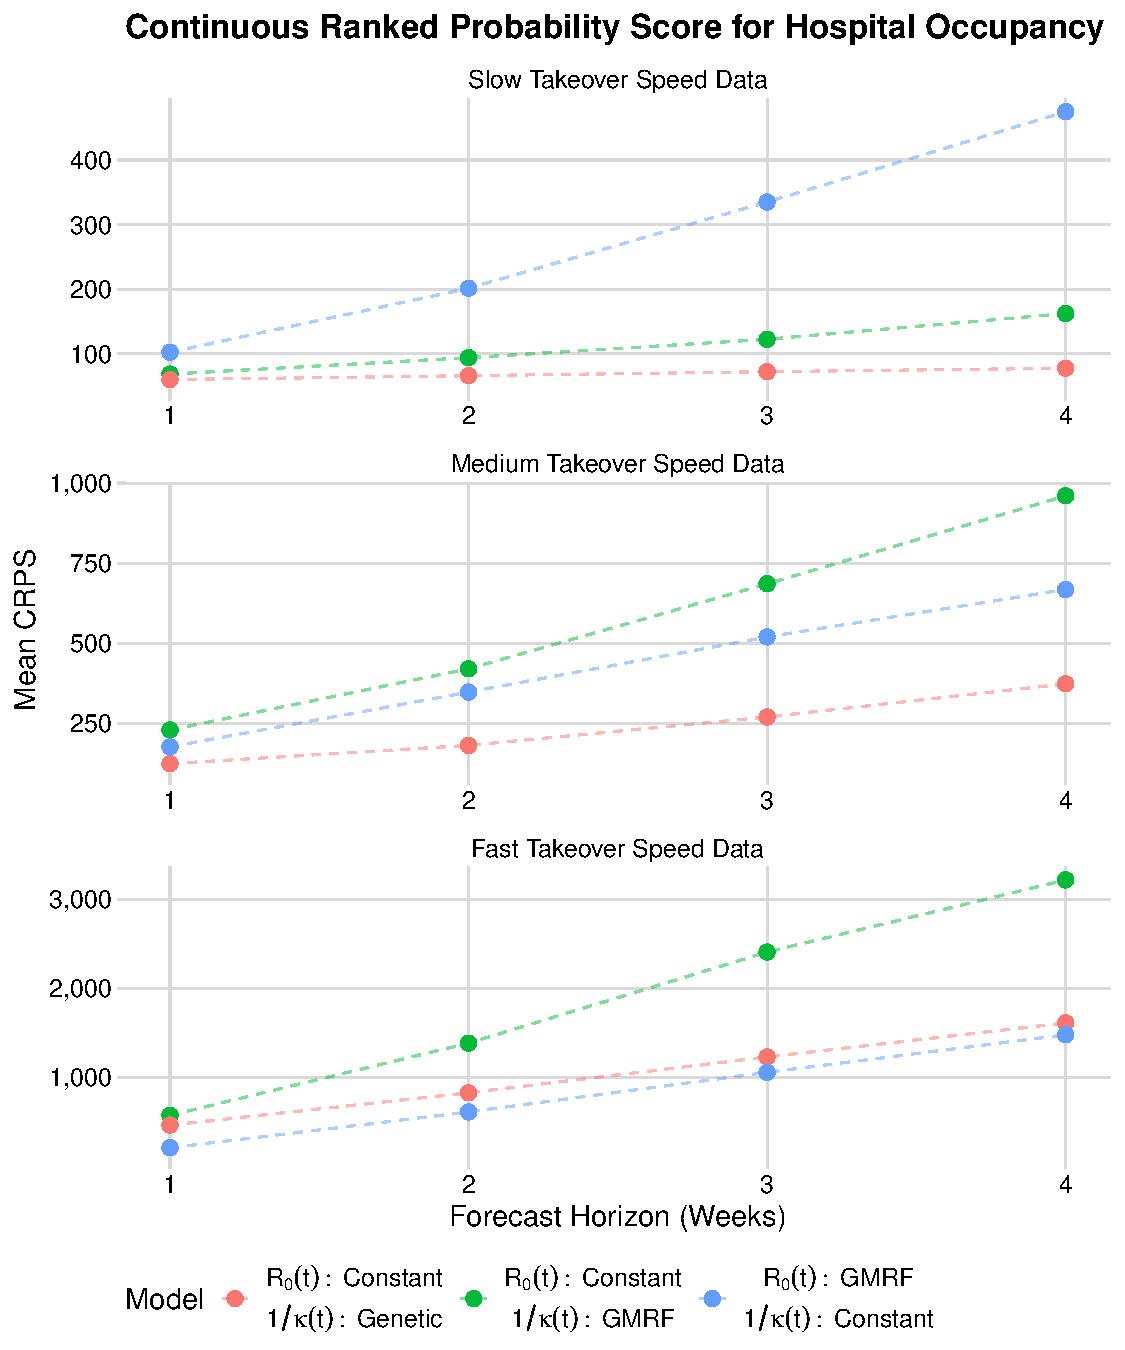
\includegraphics[width=0.75\columnwidth]{simulated_crps_comparison_dotplot_data_hospitalizations_plot}
    \caption[CRPS summaries for hospital occupancy forecasts for simulated data sets.]{CRPS summaries for hospital occupancy forecasts at 1, 2, and 4-week horizons for three simulated data sets. Lower CRPS is better.}
    \label{ch_5:fig:simulated_crps_comparison_dotplot_data_hospitalizations_plot}
\end{figure}

We also specifically assess each model's ability to estimate the timing and size of the peak hospital occupancy.
Posterior predictive intervals for the peak timing and peak value are presented in Figures~\ref{ch_5:fig:simulated_peak_assessment_time_plot} and \ref{ch_5:fig:simulated_peak_assessment_value_plot}.
In general, the model where \( 1 / \kappa(t) \) is informed by the genetic data tends to have the smallest predictive interval widths and is overconfident about peak timing and value early on, but can accurately forecast these quantities when later data is included in the model.
The model where \( R_0(t) \) follows a GMRF has the widest intervals and is, in general, under-confident about the peak timing and value, even when the peak has already passed.
The model where \( 1 / \kappa(t) \) follows a GMRF falls somewhere in the middle.

\begin{figure}
    \centering
    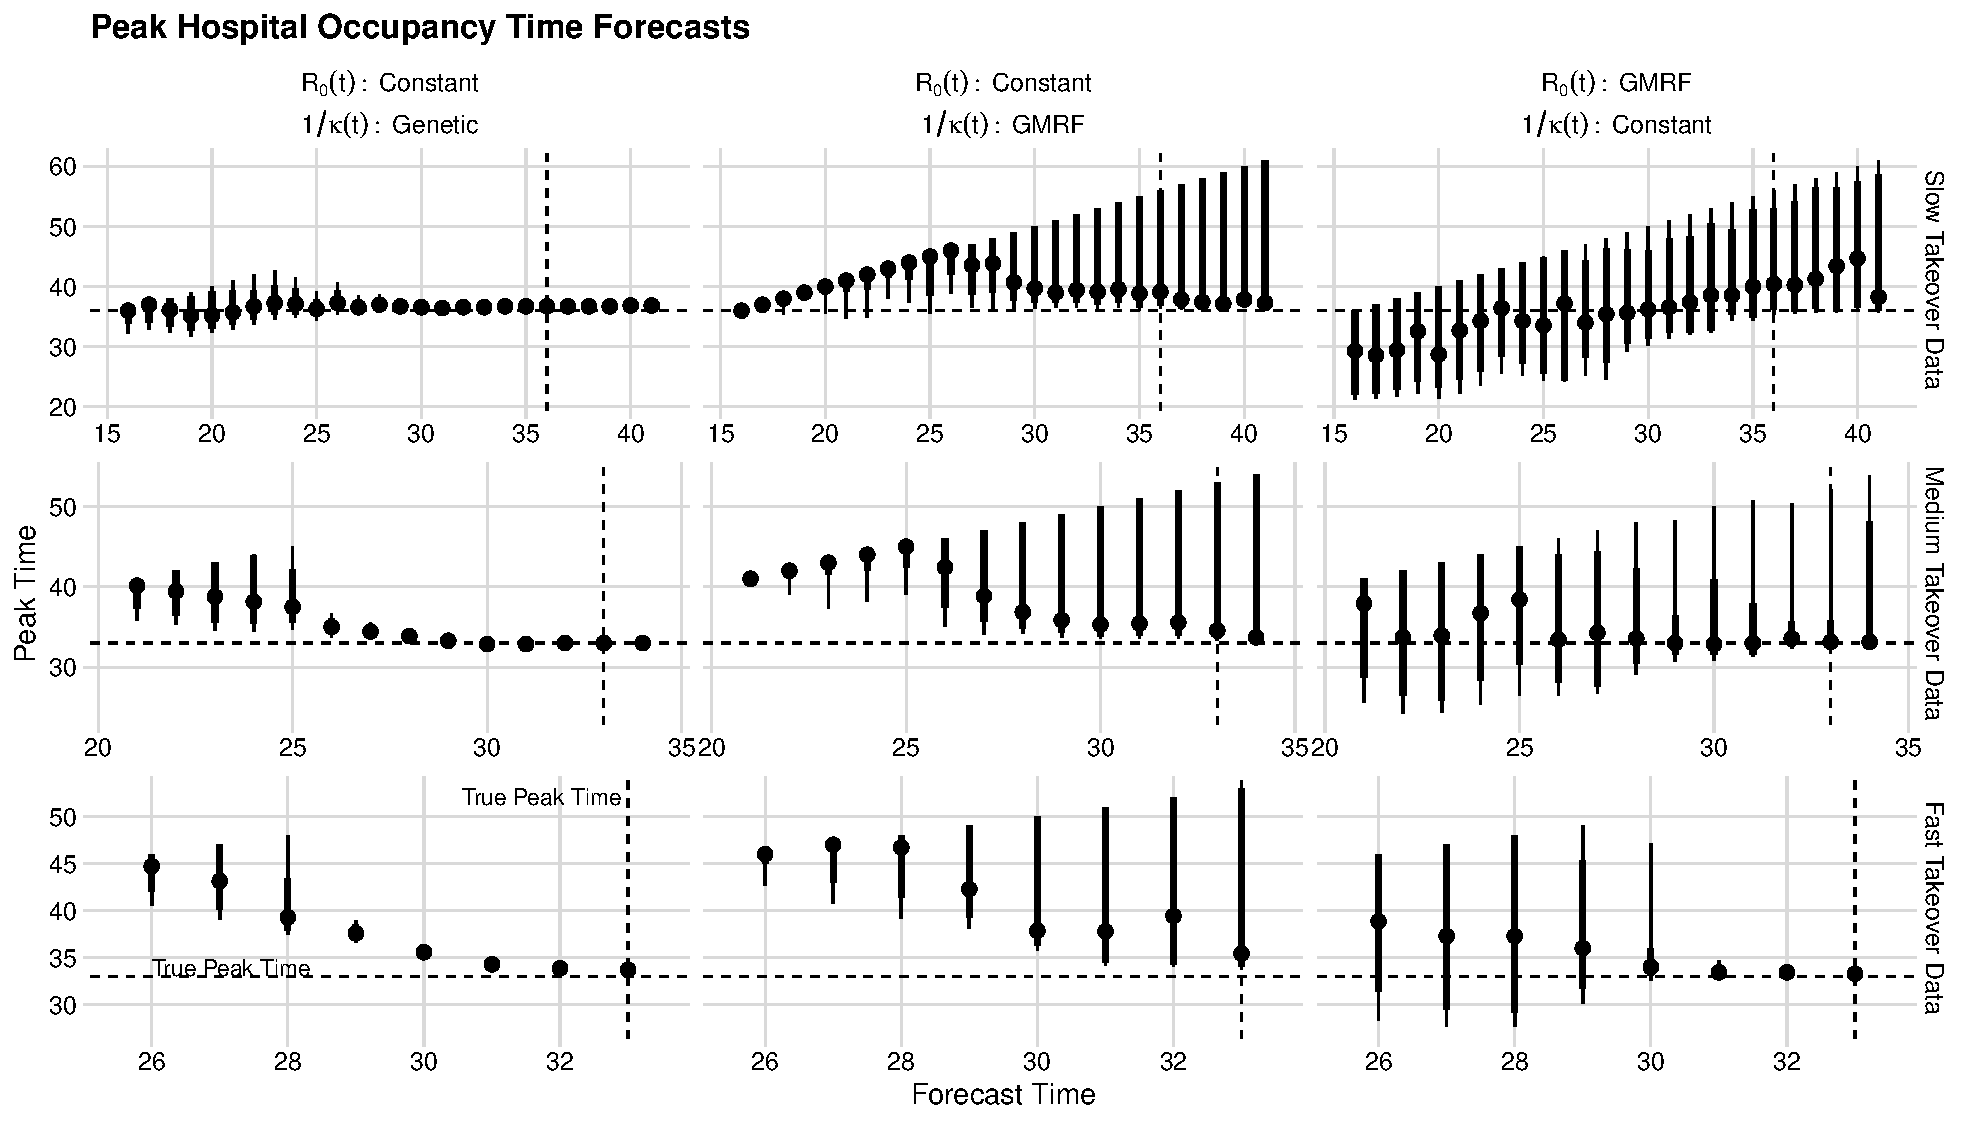
\includegraphics[width=1.0\columnwidth]{simulated_peak_assessment_time_plot}
    \caption[Posterior predictive intervals for peak hospital occupancy timing for simulated data sets.]{Posterior predictive intervals for the time at which hospital occupancy reaches its maximum in three simulated data sets.
    Dots indicate the median of the predictive distribution, while the thick and thin lines represent central 80\% and 95\% intervals, respectively.
    Horizontal and vertical dashed lines indicate the true peak hospitalization time.}
    \label{ch_5:fig:simulated_peak_assessment_time_plot}
\end{figure}

\begin{figure}
    \centering
    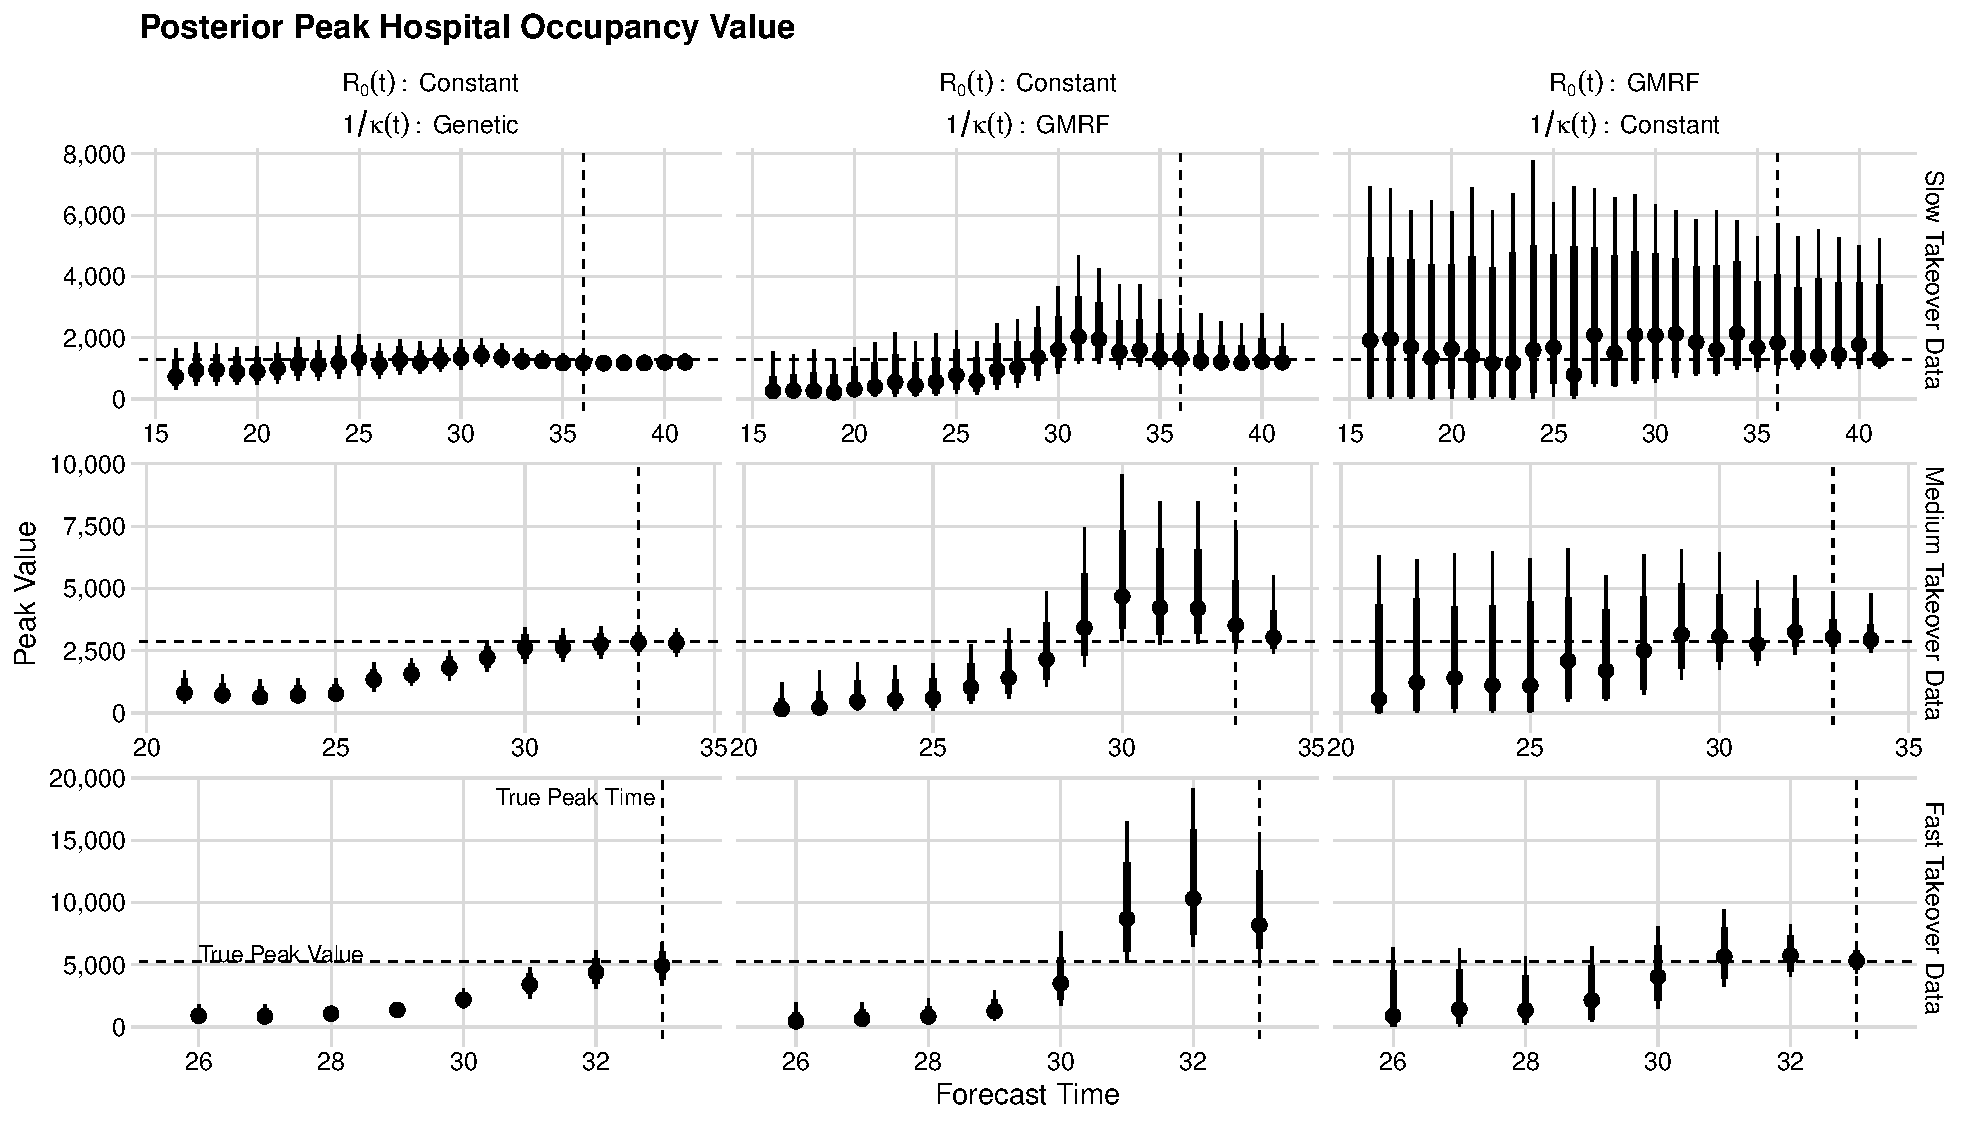
\includegraphics[width=1.0\columnwidth]{simulated_peak_assessment_value_plot}
    \caption[Posterior predictive intervals for peak hospital occupancy for simulated data sets.]{Posterior predictive intervals for the maximum hospital occupancy in three simulated data sets.
    Dots indicate the median of the predictive distribution, while the thick and thin lines represent central 80\% and 95\% intervals, respectively.
    Horizontal dashed lines indicate the true peak hospital occupancy, while the vertical dashed lines indicate the true peak hospital occupancy time.}
    \label{ch_5:fig:simulated_peak_assessment_value_plot}
\end{figure}

Summaries of the average scores for these forecasts are depicted in Figure~\ref{ch_5:fig:simulated_peak_crps_dotplot_plot}.
The score at each forecast time is shown in Figure~\ref{ch_5:fig:simulated_peak_crps_plot}.
For the slow takeover data, the model where \( 1 / \kappa(t) \) is informed by the genetic data achieves the best scores for both peak timing and value.
When the models are fit to the medium and fast takeover data, the model where \( R_0(t) \) is a priori modeled as a GMRF performs the best.

\begin{figure}
    \centering
    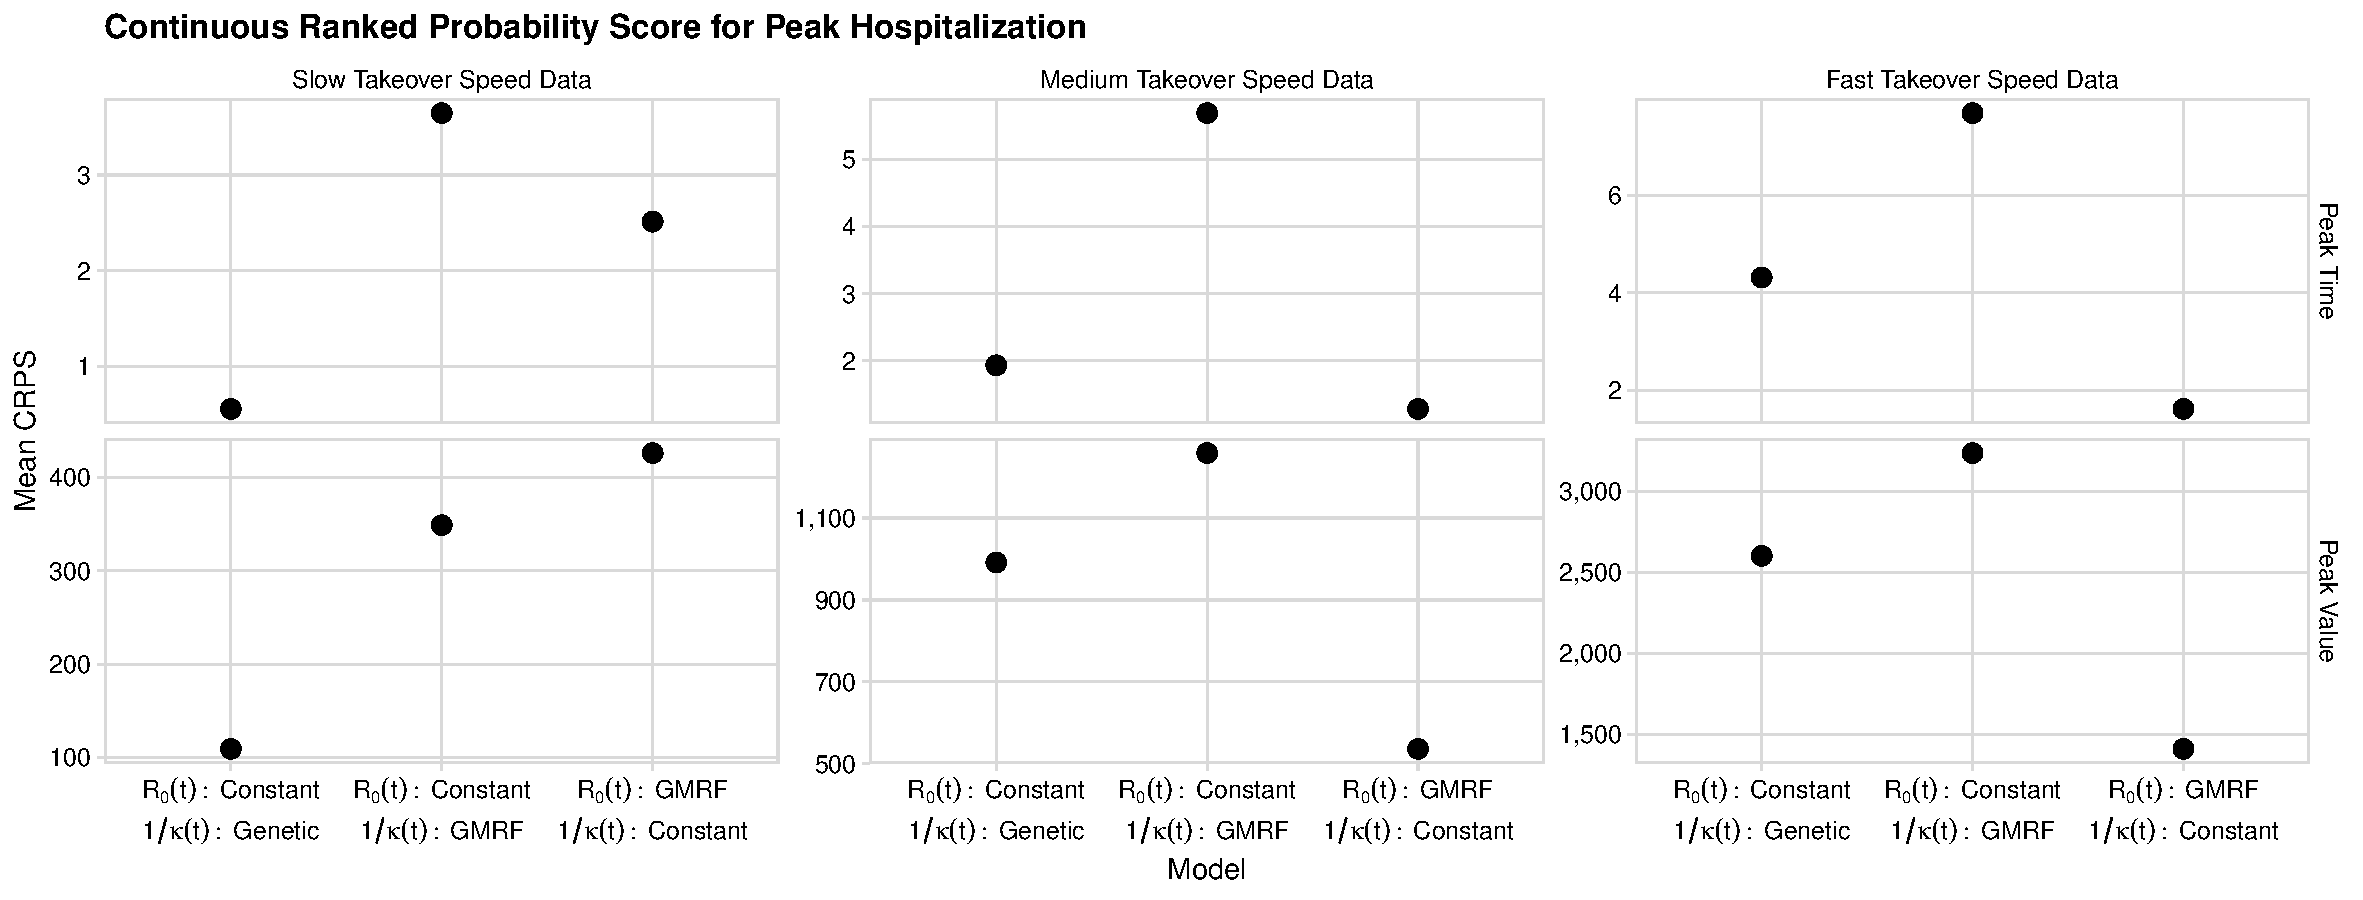
\includegraphics[width=1.0\columnwidth]{simulated_peak_crps_dotplot_plot}
    \caption[CRPS summaries for peak hospital occupancy in simulated data sets.]{CRPS summaries for peak hospital occupancy timing and size for three simulated data sets. Lower CRPS is better.}
    \label{ch_5:fig:simulated_peak_crps_dotplot_plot}
\end{figure}

Beyond the forecasting advantages, the model that uses genetic data is more computationally efficient and uses the same number of parameters, regardless of the number of observation times.
In contrast, the number of parameters in the models with GMRFs scales with the number of observation times.
A summary of the computation time required to fit models in the simulation study is presented in Table~\ref{ch_5:table:simmulation_study_cpu_time}.

\begin{table}
\caption[Computation time for models in simulation study.]{Computation time summary for all models in our simulation study.
Each fit consists of four Markov chains run in parallel to draw a total of 1000 posterior samples.}
\label{ch_5:table:simmulation_study_cpu_time}
\centering
\begin{tabular}{lrrr}
 Model & Avg. CPU Hrs & Min. CPU Hrs & Max. CPU Hrs \\ 
  \hline
\( R_0(t) \): Constant, \( 1 / \kappa(t) \): Genetic & 2.54 & 1.53 & 3.61 \\ 
\( R_0(t) \): Constant, \( 1 / \kappa(t) \): GMRF & 5.47 & 2.93 & 8.63 \\ 
\( R_0(t) \): GMRF, \( 1 / \kappa(t) \): Constant & 11.05 & 4.15 & 21.70
\end{tabular}
\end{table}

\subsection{Application to California data}
\label{ch_5:subsec:application}

In our real data application, we focus on modeling the wave of cases, hospitalizations, ICU admissions, and deaths associated with the first Omicron variant of SARS-CoV-2 in California.
This wave lasted from roughly December 2021 to March 2022, but we use data beginning in May 2021 to forecast the wave, as this time period includes the previous wave of cases.
We fit models to both Orange County data and statewide California data.
The time series of daily counts of cases, hospital occupancy, ICU occupancy, and deaths due to COVID-19 are provided by the California Department of Public of Health, and published on the California Open Data Portal (\url{https://data.ca.gov}).
Additionally, the daily counts of sequenced viruses, aggregated by pango lineage \citep{pango}, are provided by the Global Initiative on Sharing All Influenza Data (GISAID) \citep{shu2017gisaid} and made available via Outbreak.info \citep{Gangavarapu2023}.
To match the format described in Section~\ref{ch_5:sec:methods}, the lineages are further aggregated into those that begin with ``BA.1" (e.g. BA.1, BA.1.1, BA.1.17.2) and those that do not.
The BA.1 sequences are the ``novel" variant, and the BA.1 and non-BA.1 sequences are summed together as ``all" variants.
The non-genetic time series are aggregated at a weekly level, while the genetic data is used at a daily resolution, beginning about one week before the first novel variant is observed.
Because the BA.1 variant becomes dominant so quickly, the daily observation of the genetic data is crucial to capture this change, while the weekly observation of other data streams prevents us from needing to account for data inconsistencies, like the ``weekend effect" where fewer cases are reported on weekends.

Figure~\ref{ch_5:fig:california_binned_data_plot} shows the binned data at the statewide level, while Figure~\ref{ch_5:fig:orange_county_binned_data_plot} displays the binned data from Orange County.
The gray highlighted regions indicate the times for which we produce forecasts.
We note that, while the peak weekly case count in the BA.1 wave is about six times higher than the first wave depicted in the figure, the peak hospitalizations are only twice as high in the second wave, and the peak ICU occupancy is only about 20\% higher in the second wave.
This is a clear departure from the models we fit in our simulation study, where the second peak's height compared to the first peak is the same for all data streams.
Because of this, we chose to fit the same models as in the simulation study, but modified them to also include modeling the case detection rate, \( \rho^W(t) \), with a GMRF.
In reality, the reasoning for the changing relationship between the peaks is complex and difficult to untangle, even in retrospect.
It is likely that some combination of partial protection from previous infections or vaccinations and possible less inherent propensity for severe outcomes in the Omicron variant are at play.
Anticipating and modeling this scenario in a real forecasting scenario with a novel variant would be extremely difficult, so we chose to incorporate some additional flexibility into the model in a place that could be realistic and useful.

\begin{figure}
    \centering
    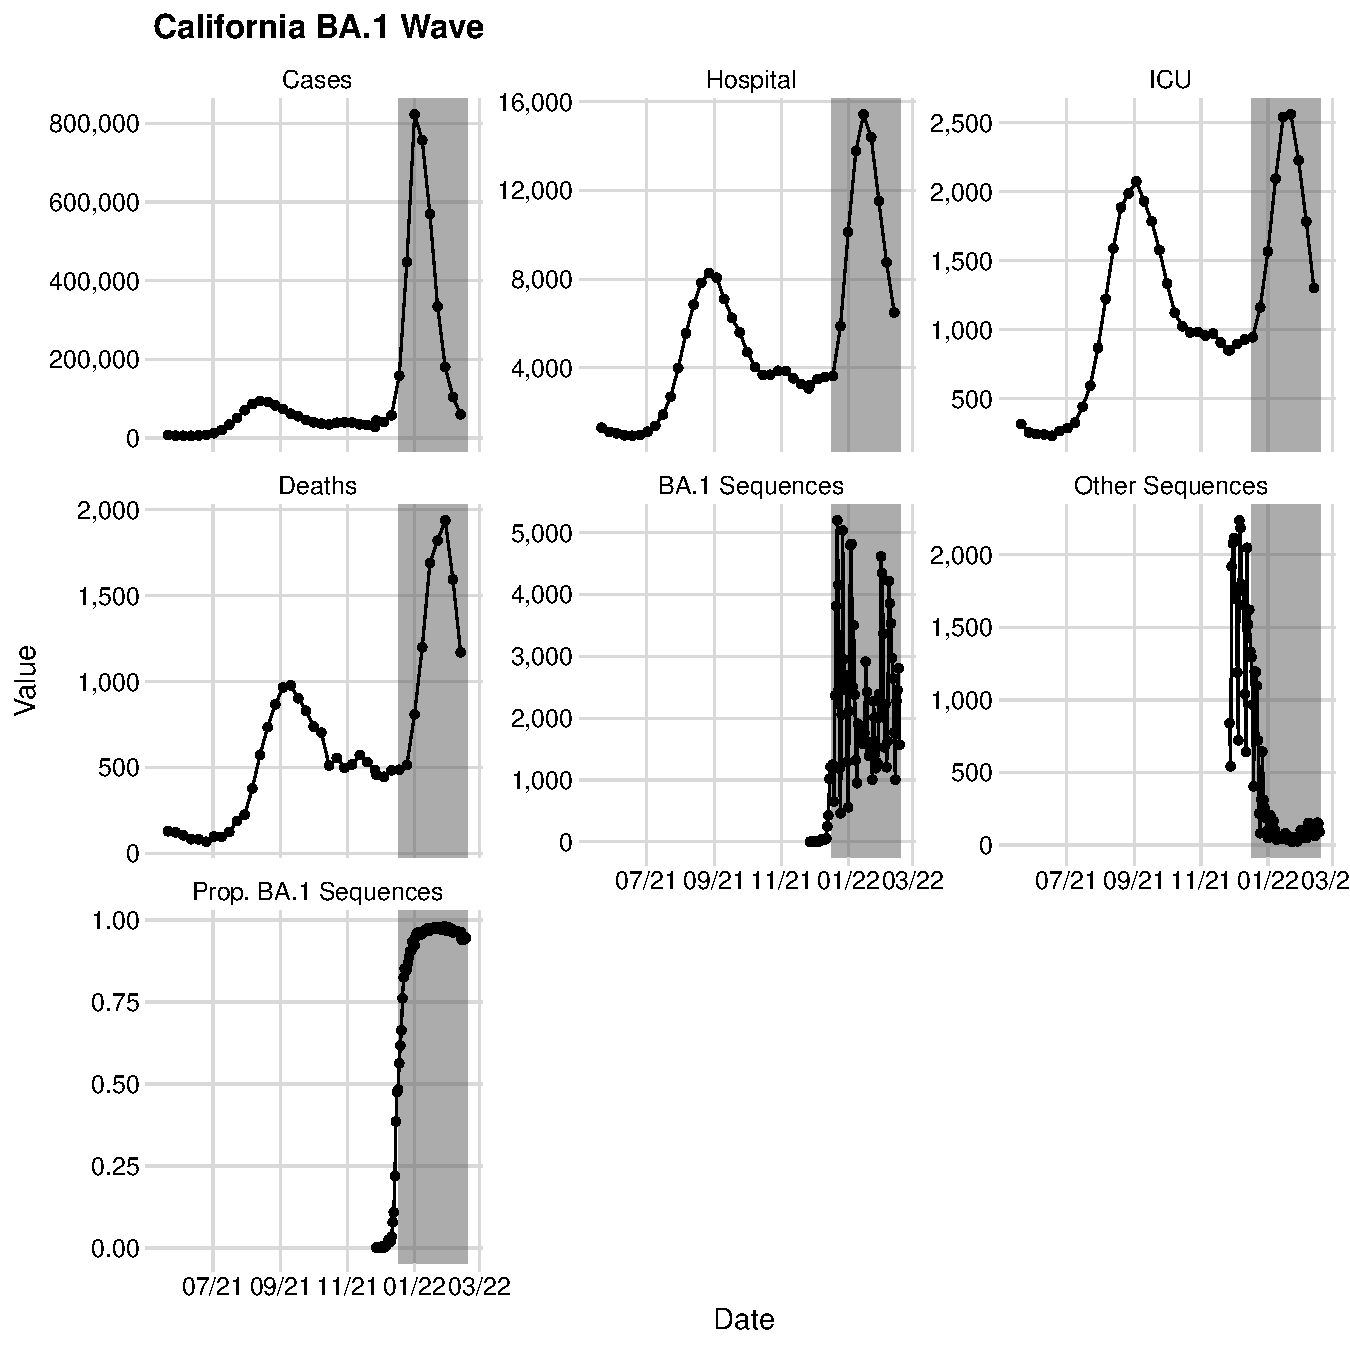
\includegraphics[width=1.0\columnwidth]{california_binned_data_plot.pdf}
    \caption[COVID-19 surveillance data from California.]{
COVID-19 surveillance data from California.
The plots show weekly counts of cases, hospital and ICU occupancy of patients with COVID-19, reported deaths due to COVID-19, as well as counts of virus sequences for Omicron BA.1 and all lineages, and the proportion of BA.1 lineages.
The gray highlighted regions indicate the times for which we produce forecasts.}
    \label{ch_5:fig:california_binned_data_plot}
\end{figure}

\begin{figure}
    \centering
    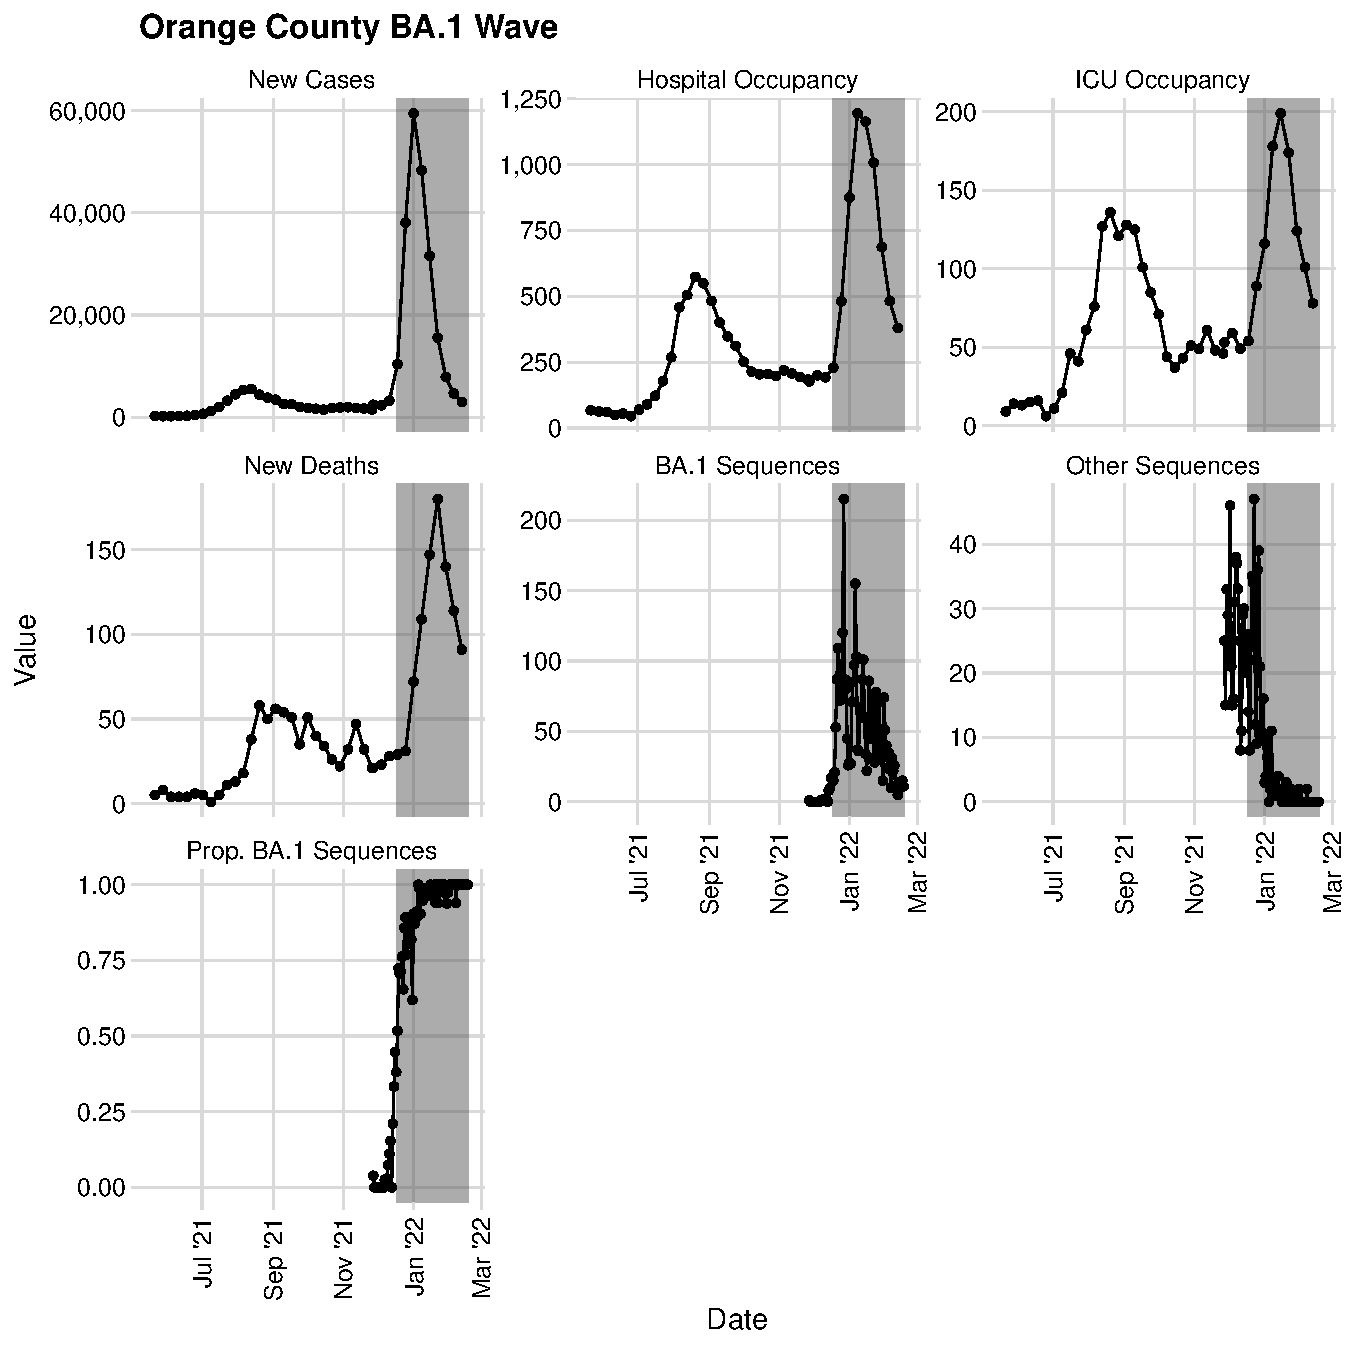
\includegraphics[width=1.0\columnwidth]{orange_county_binned_data_plot.pdf}
    \caption[COVID-19 surveillance data from Orange County, California.]{
COVID-19 surveillance data from Orange County, CA.
The plots show weekly counts of cases, hospital and ICU occupancy of patients with COVID-19, reported deaths due to COVID-19, as well as counts of virus sequences for Omicron BA.1 and all lineages, and the proportion of BA.1 lineages.
The gray highlighted regions indicate the times for which we produce forecasts.}
    \label{ch_5:fig:orange_county_binned_data_plot}
\end{figure}

The priors used for our models are presented in Table~tk.
For each data set, we used four Markov chains run in parallel to draw a total of 1000 posterior samples.
As in the simulation study, in the main text, we focus on results related to hospital occupancy, but present results for cases, ICU occupancy, and deaths in Section~\ref{ch_5:sec:real_cases_icu_death}.
In general, these results exhibit the similar patterns as observed in the hospitalization results.

Figures~\ref{ch_5:fig:real_data_forecast_comparison_data_hospitalizations_California_plot} and \ref{ch_5:fig:real_data_forecast_comparison_data_hospitalizations_Orange_plot} show the 1, 2, and 4-week ahead forecasts for hospital occupancy in Orange County and California, respectively.
For both data sets, we note that one-week ahead forecasts match the data quite closely for the models that do not use the genetic data, but the model where \( 1 / \kappa(t) \) is informed by the genetic data exhibits comparatively wider credible intervals.
As the forecast horizon increases, the two models where \( 1 / \kappa(t) \) varies in time can correctly identify the peak of the hospital occupancy, while the model where \( 1 / \kappa(t) \) is constant greatly overestimates the peak.
These observations are reflected in Figure~\ref{ch_5:fig:real_data_crps_comparison_dotplot_data_hospitalizations_plot}, where we observe that the model where \( 1 / \kappa(t) \) is informed by genetic data achieves the lowest average CRPS values at forecast horizons greater than one week, and the model where \( 1 / \kappa(t) \) is constant achieves the highest CRPS values.
Analogous figures for the other data streams are presented in Figures~\ref{ch_5:fig:real_data_crps_comparison_dotplot_data_new_cases_plot}--\ref{ch_5:fig:real_data_crps_comparison_dotplot_data_new_deaths_plot}.
We show the individual scores for each forecast in Figures~\ref{ch_5:fig:real_data_crps_comparison_data_new_cases_plot}--\ref{ch_5:fig:real_data_crps_comparison_data_new_deaths_plot}.
In Figures~\ref{ch_5:fig:real_data_peak_assessment_time_plot} and \ref{ch_5:fig:real_data_peak_assessment_value_plot}, we present posterior predictive intervals for the peak timing and peak value for hospital occupancy.
One again, the models where \( 1 / \kappa(t) \) varies in time are shown to be superior, with narrower credible intervals near the observed value in the data.
In particular, the model where \( 1 / \kappa(t) \) is informed by genetic data appears to be best at forecasting the time of the hospital occupancy peak.
This is demonstrated in Figure~\ref{ch_5:fig:real_data_peak_crps_dotplot_plot}, which shows a summary of the average CRPS values for forecasts of peak hospital occupancy time and amount.
Individual CRPS values for each forecast of a peak hospital occupancy time and amount are presented in Figure~\ref{ch_5:fig:real_data_peak_crps_plot}.

\begin{figure}
    \centering
    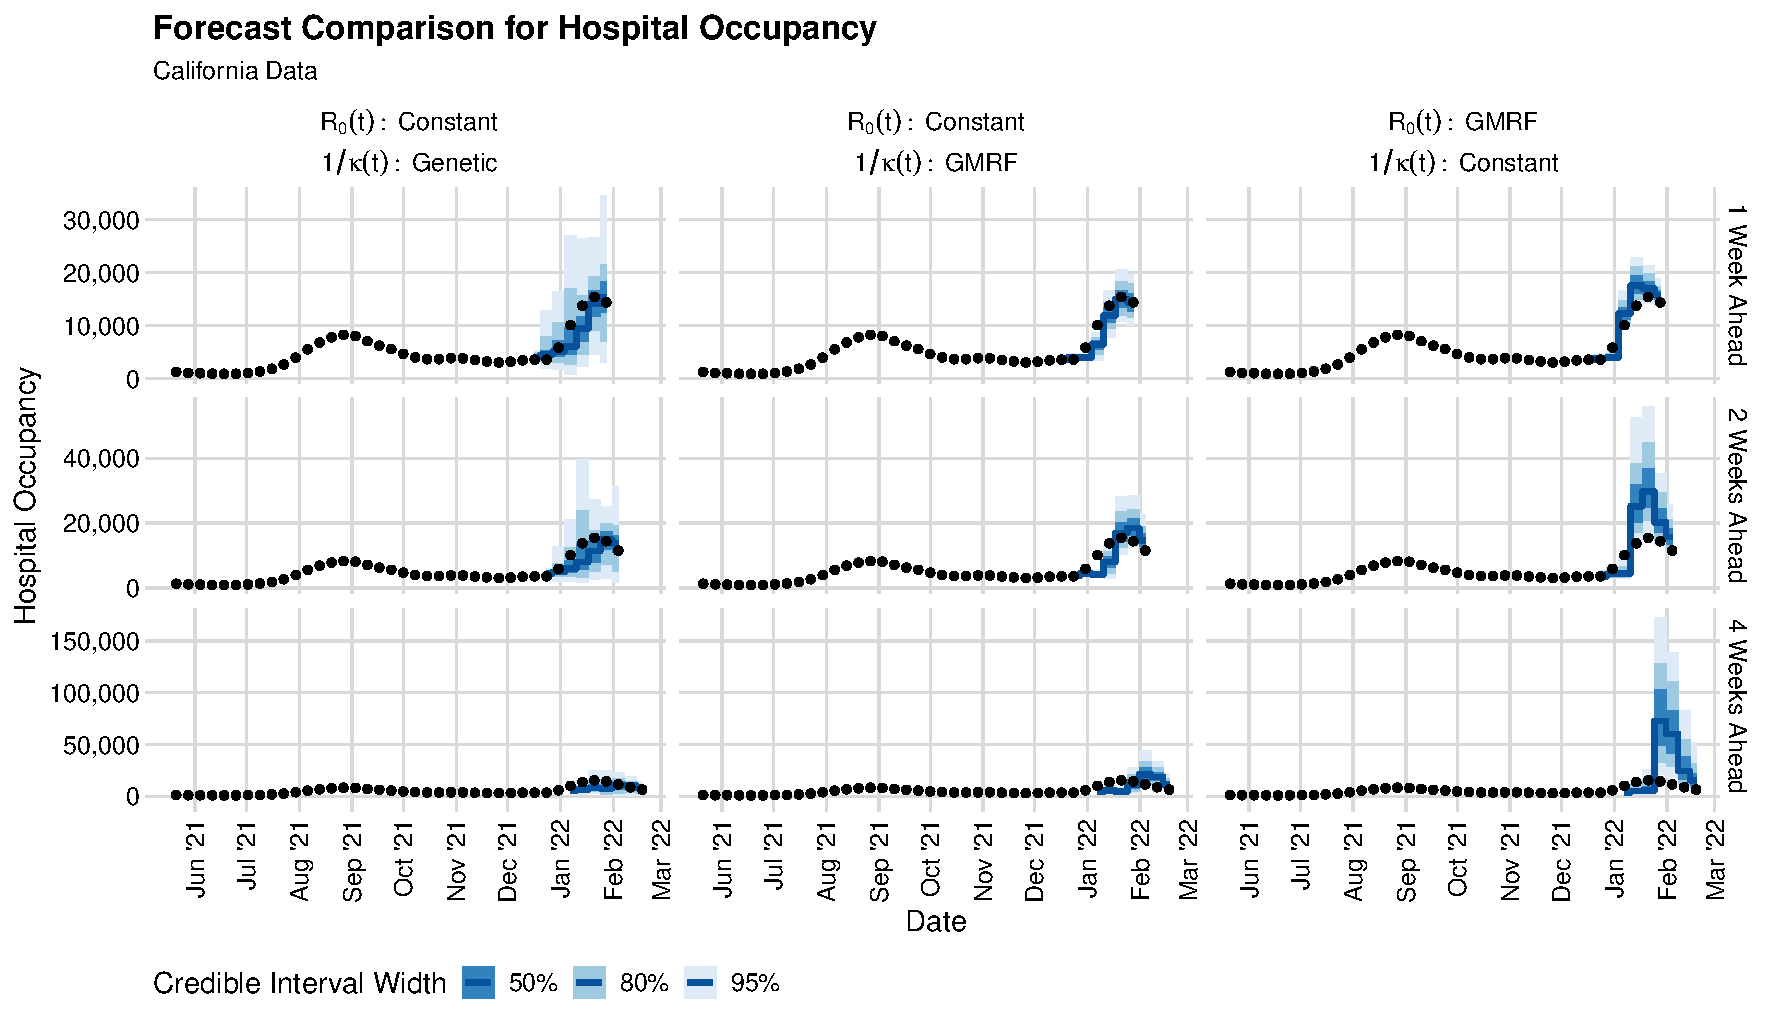
\includegraphics[width=1.0\columnwidth]{real_data_forecast_comparison_data_hospitalizations_California_plot}
    \caption[Hospital occupancy forecasts for California data.]{Hospital occupancy forecasts from three models at 1, 2, and 4-week forecast horizons for the California data.}
    \label{ch_5:fig:real_data_forecast_comparison_data_hospitalizations_California_plot}
\end{figure}

\begin{figure}
    \centering
    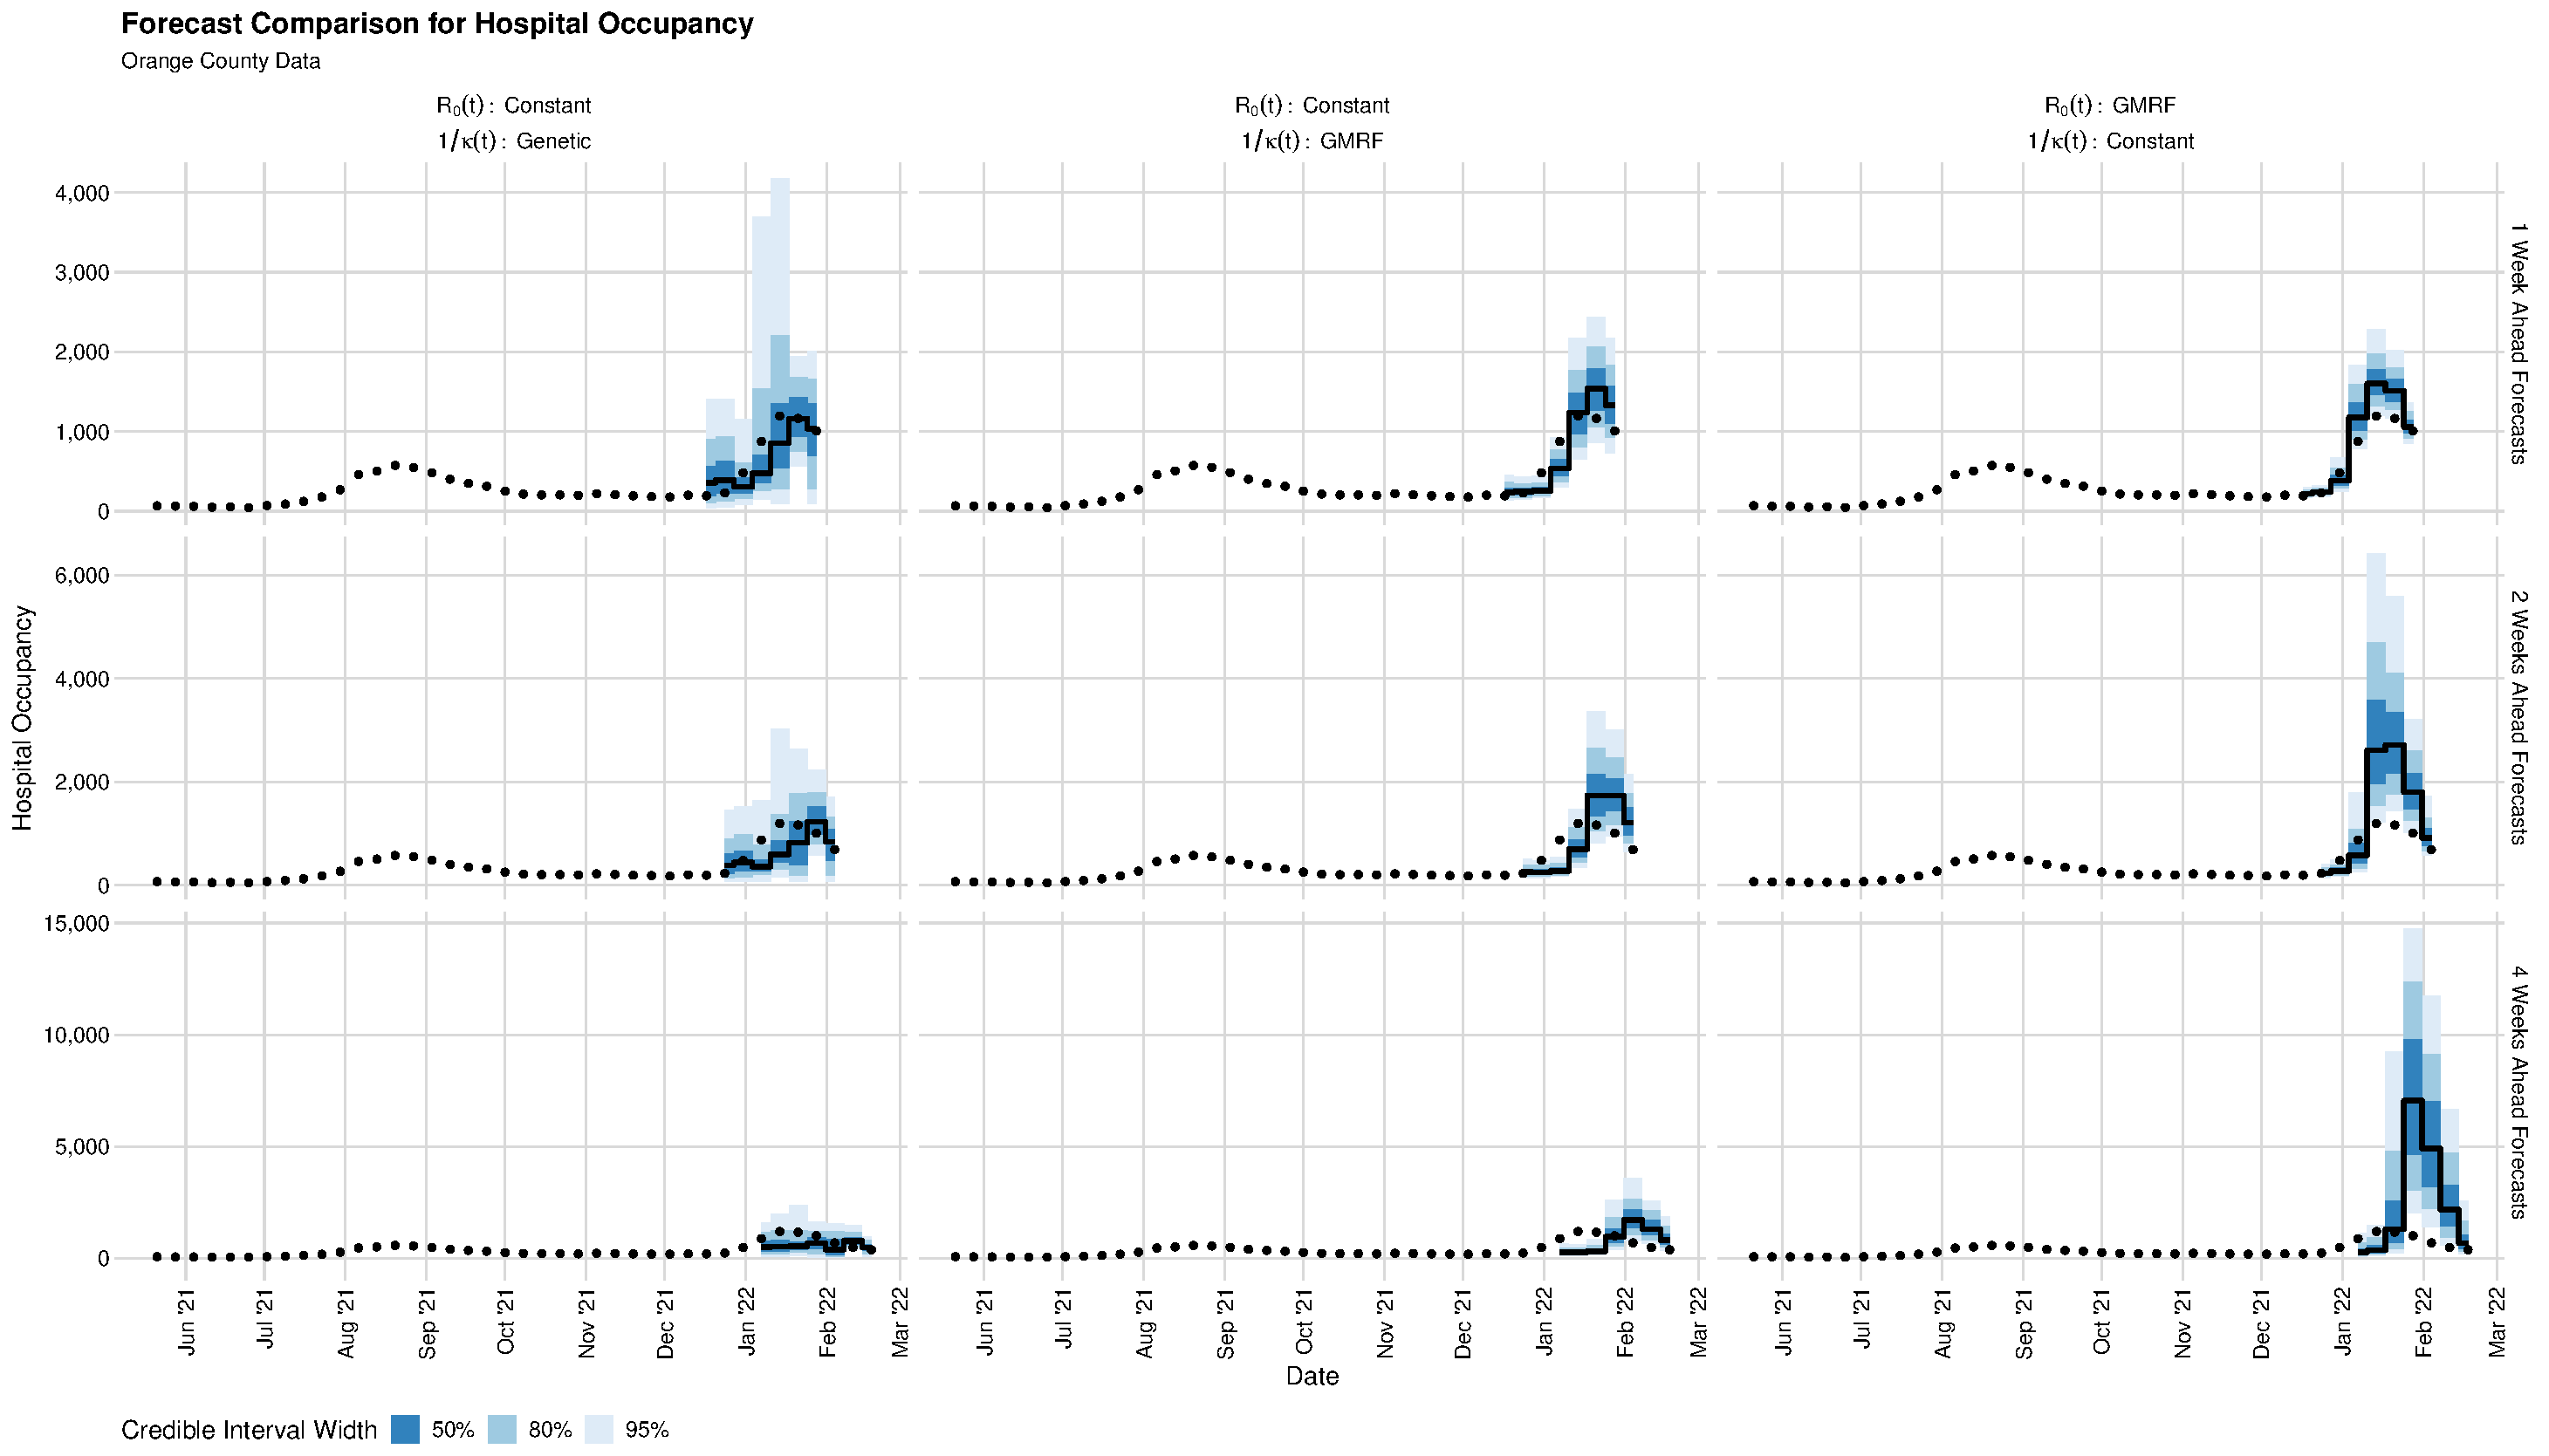
\includegraphics[width=1.0\columnwidth]{real_data_forecast_comparison_data_hospitalizations_Orange_plot}
    \caption[Hospital occupancy forecasts for Orange County data.]{Hospital occupancy forecasts from three models at 1, 2, and 4-week forecast horizons for the Orange County data.}
    \label{ch_5:fig:real_data_forecast_comparison_data_hospitalizations_Orange_plot}
\end{figure}

\begin{figure}
    \centering
    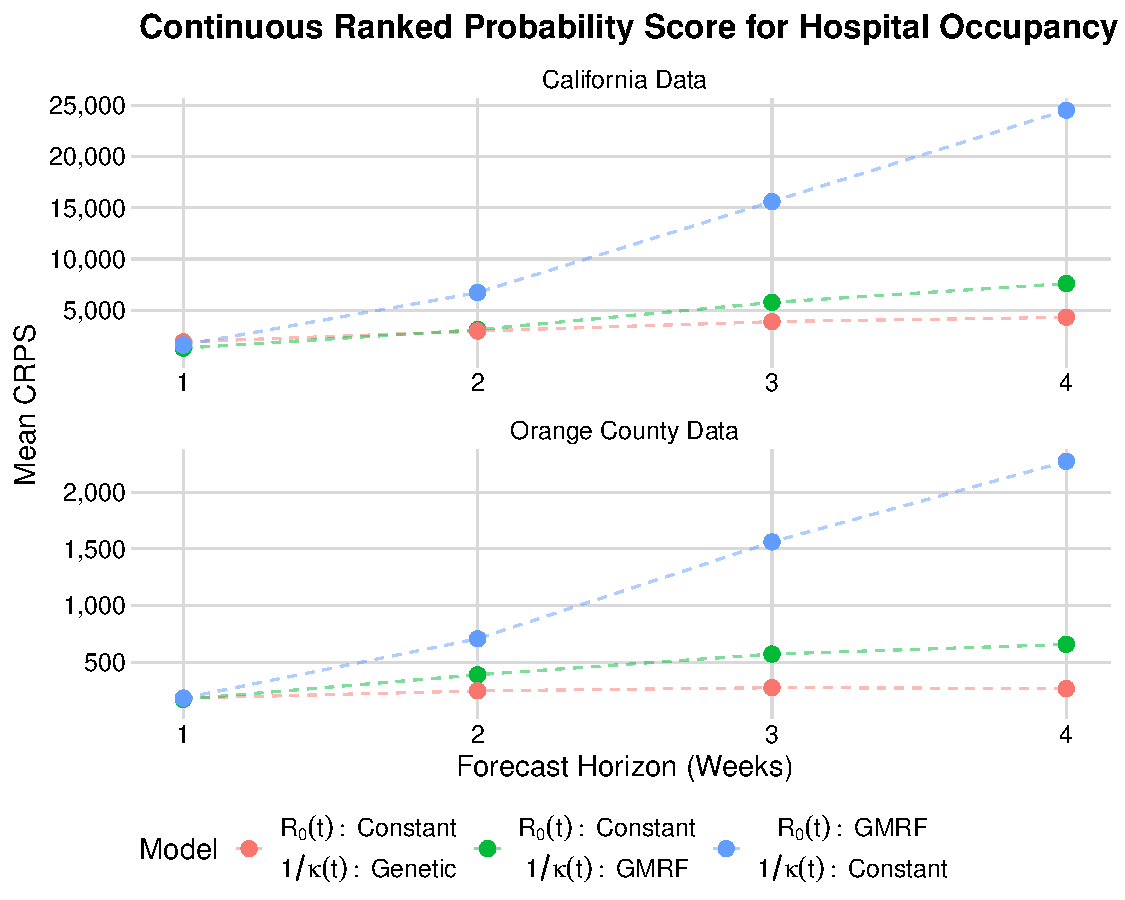
\includegraphics[width=1.0\columnwidth]{real_data_crps_comparison_dotplot_data_hospitalizations_plot}
    \caption[CRPS summaries for hospital occupancy forecasts for real data sets.]{CRPS summaries for hospital occupancy forecasts at 1, 2, and 4-week horizons for California and Orange County data sets. Lower CRPS is better.}
    \label{ch_5:fig:real_data_crps_comparison_dotplot_data_hospitalizations_plot}
\end{figure}

\begin{figure}
    \centering
    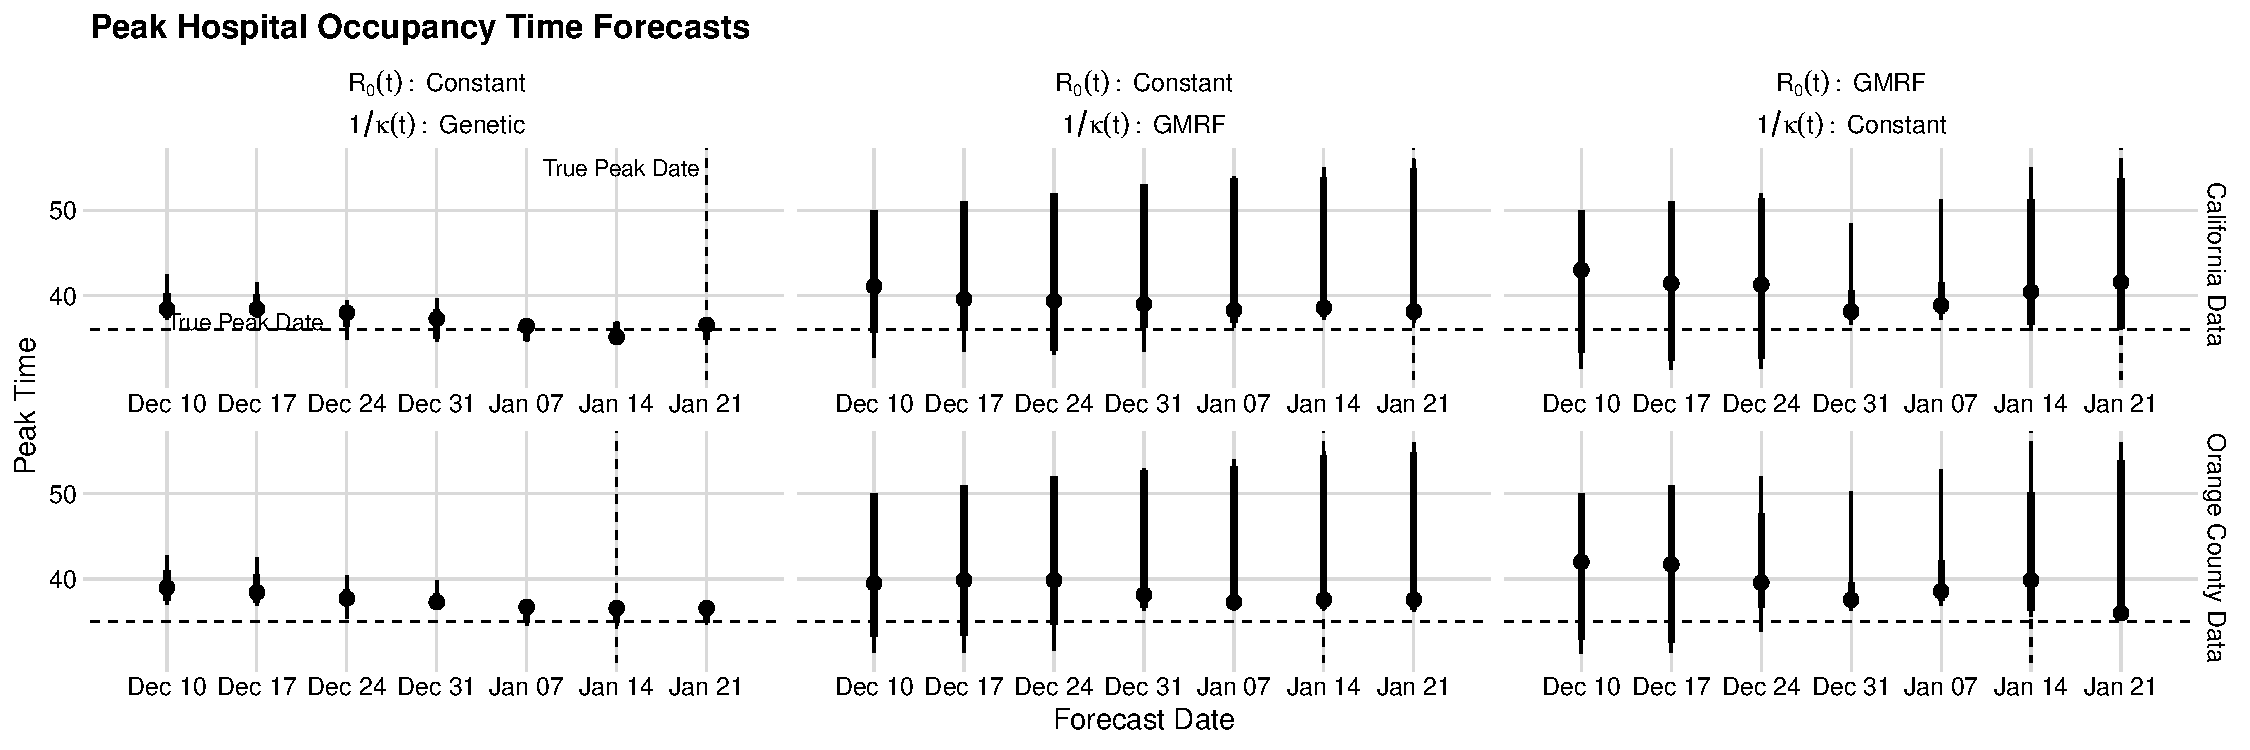
\includegraphics[width=1.0\columnwidth]{real_data_peak_assessment_time_plot}
    \caption[Posterior predictive intervals for peak hospital occupancy timing for real data sets.]{Posterior predictive intervals for the time at which hospital occupancy reaches its maximum in California and Orange County data sets.
    Dots indicate the median of the predictive distribution, while the thick and thin lines represent central 80\% and 95\% intervals, respectively.
    Horizontal and vertical dashed lines indicate the true peak hospitalization time.}
    \label{ch_5:fig:real_data_peak_assessment_time_plot}
\end{figure}

\begin{figure}
    \centering
    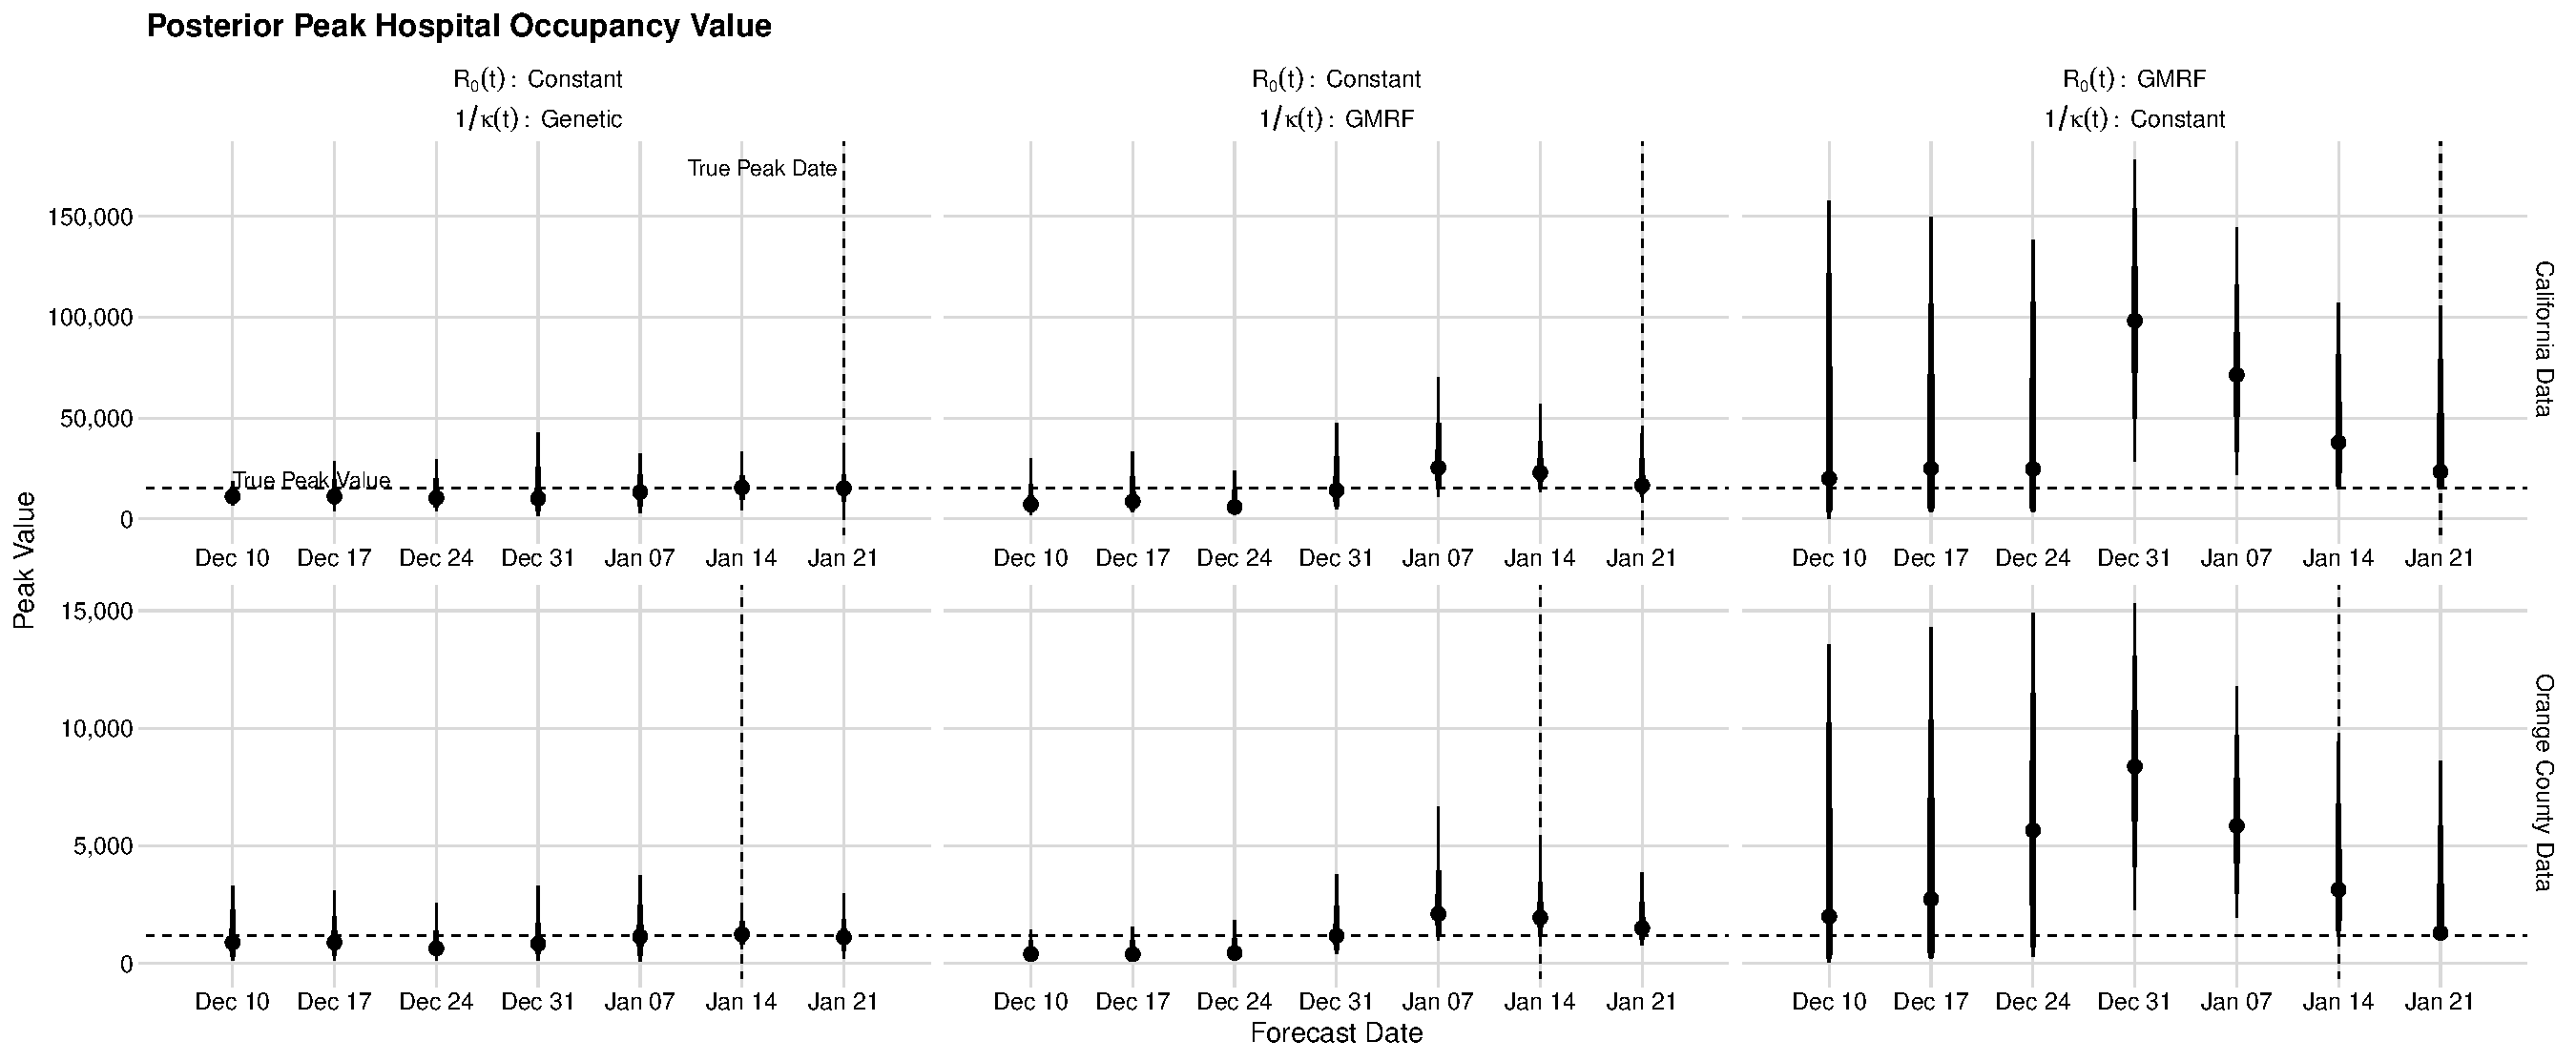
\includegraphics[width=1.0\columnwidth]{real_data_peak_assessment_value_plot}
    \caption[Posterior predictive intervals for peak hospital occupancy for real data sets.]{Posterior predictive intervals for the maximum hospital occupancy in Orange County and California  data sets.
    Dots indicate the median of the predictive distribution, while the thick and thin lines represent central 80\% and 95\% intervals, respectively.
    Horizontal dashed lines indicate the true peak hospital occupancy, while the vertical dashed lines indicate the true peak hospital occupancy time.}
    \label{ch_5:fig:real_data_peak_assessment_value_plot}
\end{figure}

\begin{figure}
    \centering
    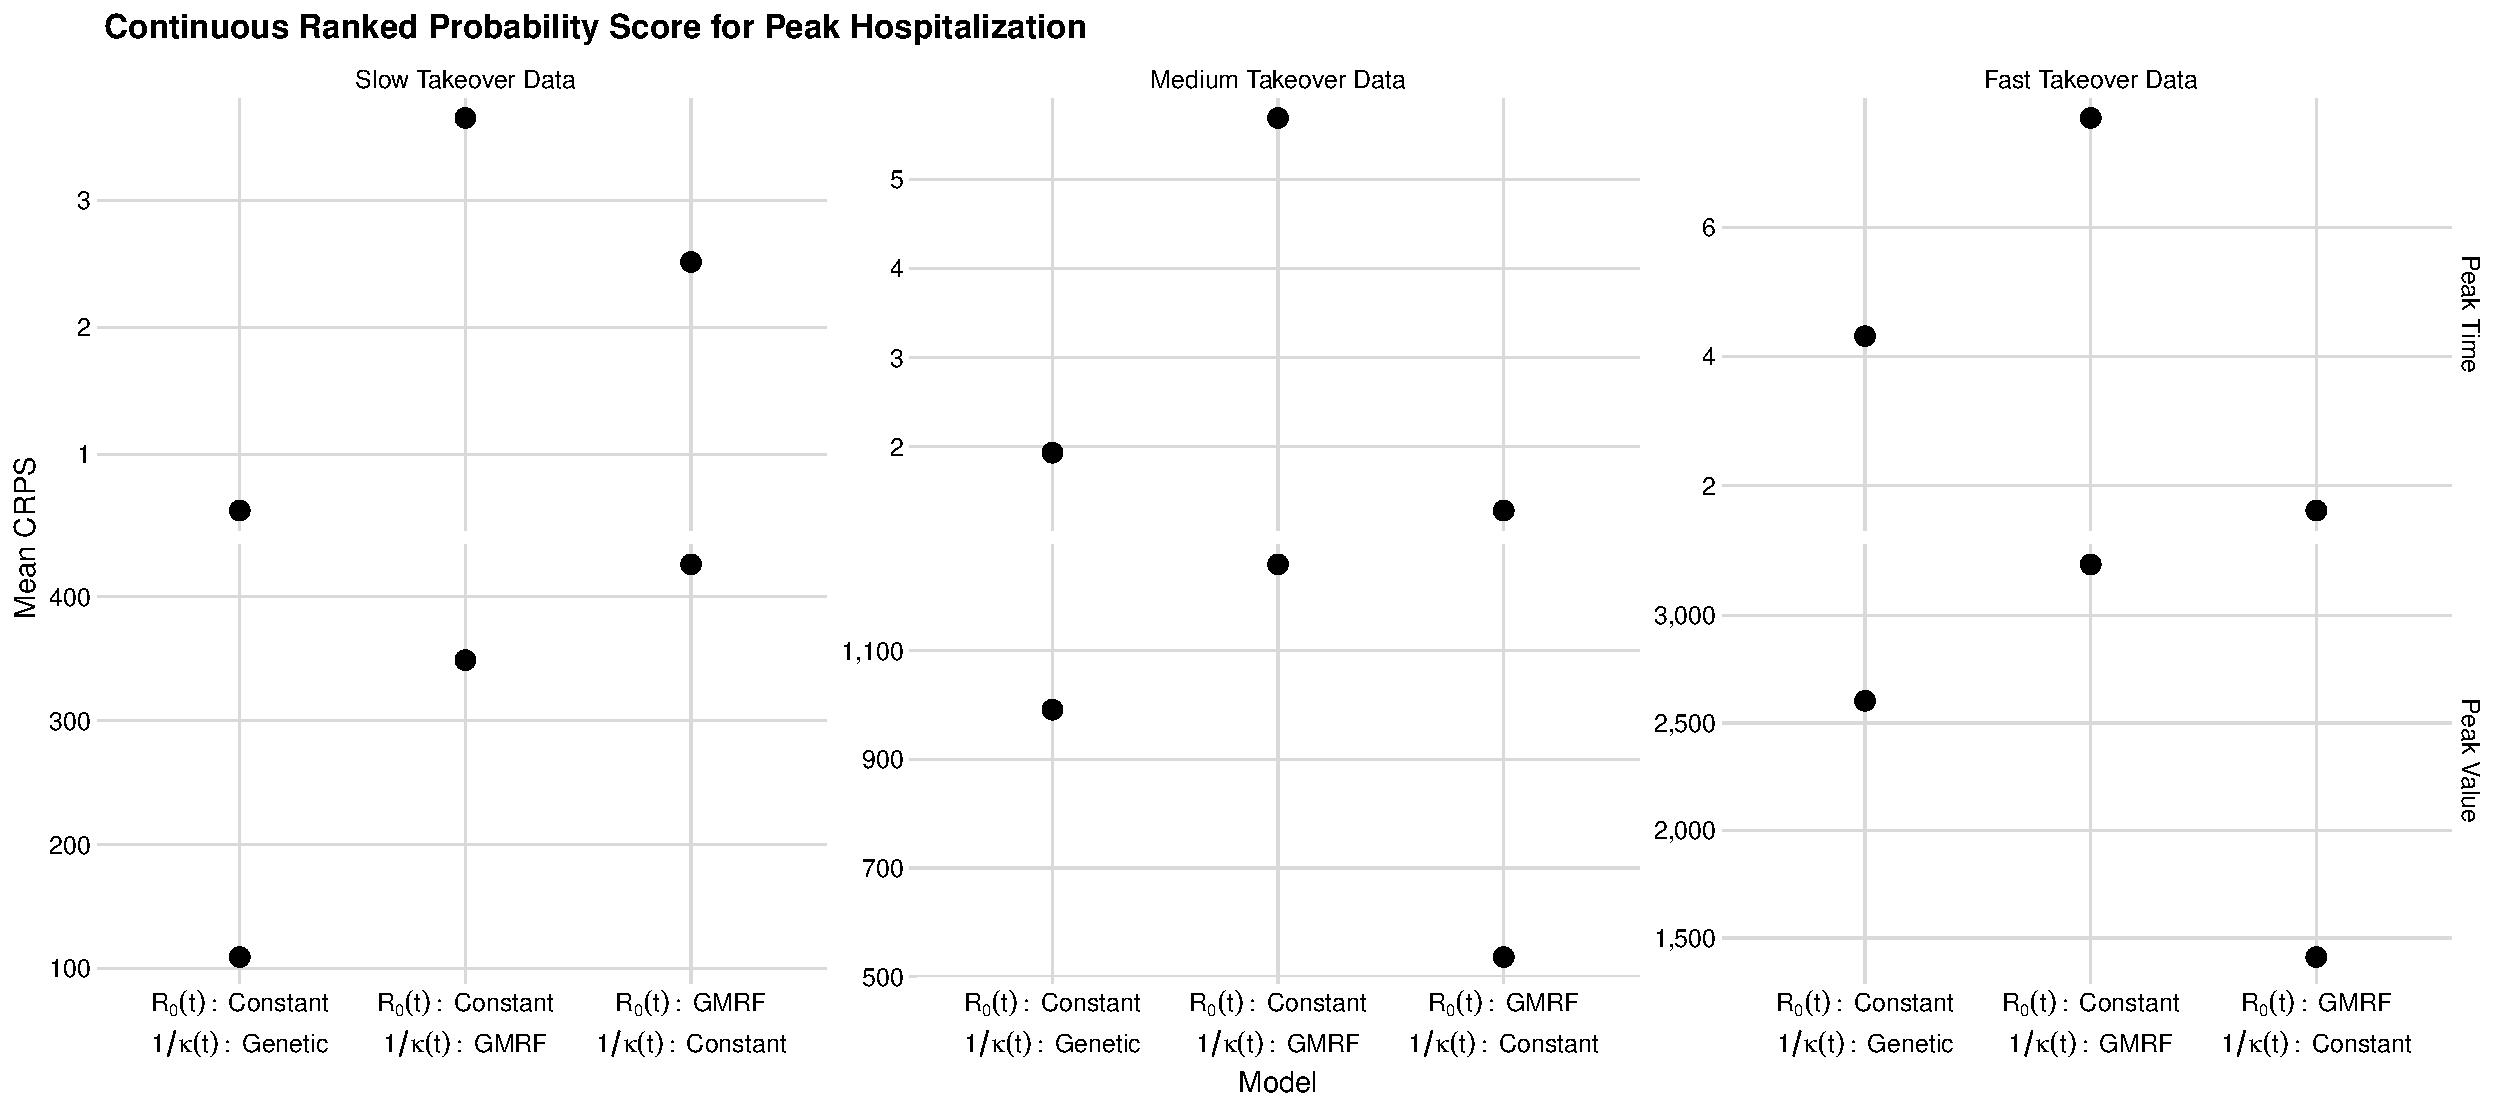
\includegraphics[width=1.0\columnwidth]{real_data_peak_crps_dotplot_plot}
    \caption[CRPS summaries for peak hospital occupancy in real data sets.]{CRPS summaries for peak hospital occupancy timing and size in California and Orange County data sets. Lower CRPS is better.}
    \label{ch_5:fig:real_data_peak_crps_dotplot_plot}
\end{figure}

As in the simulation study, the model that uses genetic data is more computationally efficient than the models that use more GMRFs.
A summary of the computation time required to fit models in the simulation study is presented in Table~\ref{ch_5:table:real_data_cpu_time}

\begin{table}
\caption[Computation time for models in real data application.]{Computation time summary for all models in our real data application.
Each fit consists of four Markov chains run in parallel to draw a total of 1000 posterior samples.}
\label{ch_5:table:real_data_cpu_time}
\centering
\begin{tabular}{lrrr}
 Model & Avg. CPU Hrs & Min. CPU Hrs & Max. CPU Hrs \\ 
  \hline
\( R_0(t) \): Constant, \( 1 / \kappa(t) \): Genetic & 4.47 & 2.00 & 9.12 \\ 
\( R_0(t) \): Constant, \( 1 / \kappa(t) \): GMRF & 16.17 & 9.10 & 28.01 \\ 
\( R_0(t) \): GMRF, \( 1 / \kappa(t) \): Constant & 30.98 & 22.44 & 41.15
\end{tabular}
\end{table}

\section{Discussion}
\label{ch_5:sec:discussion}

We developed a Bayesian model that integrates time series of cases, hospitalizations, ICU admissions, and deaths, as well as genetic data to produce forecasts during time periods where a novel virus variant becomes dominant.
Our approach is based on the idea that the introduction of a novel variant leads to increased infections, primarily due to immune escape.
As such, we allow the parameter in our model reflecting the average immune duration to change over time and consider modeling this time-varying parameter both parametrically using genetic data, and non-parametrically.
We applied our model to simulated data sets as well as real data from the Omicron wave in Orange County and the state of California, with a particular focus on forecasting hospital occupancy.
We compare our models with time-varying immune duration to a standard model where the basic reproduction number varies in time and is modeled non-parametrically.
In simulated data sets, the model where the time-varying immune duration is informed by genetic data produces superior forecasts when the new variant becomes dominant at a ``slow" or ``medium" pace (24 or 13 weeks to go from 1\% to 99\% of sequences, respectively).
When the new variant becomes dominant quickly (6 weeks), this model is competitive with the model where the basic reproduction number is modeled non-parametrically, which performs the best.
In the real data scenarios, the model where the time-varying immune duration is informed by genetic data is shown to be especially useful for forecasting the timing and size of peak hospital occupancy, a metric that is of great interest to public health agencies.

Despite these advancements, some potential issues remain unaddressed by our model.
First, our model asserts that a novel variant must lead to reduced immunity in the population, and therefore cause a second wave.
In reality, a variant may become dominant simply due to genetic drift and not be accompanied by an increase in cases, hospitalizations or deaths.
Importantly, we assess our model only on retrospective data and do not account for reporting delays.
In a real-time forecasting, it should be possible to obtain up-to-date counts of hospital and ICU occupancy, but case, death, and sequence counts may be reported with significant delays.
Since our likelihood for the new variant sequences is conditional on the total number of sequences, this data does not directly impact our estimates of latent incidence, and it may not be necessary to model these delays for the genetic data.
In contrast, the case and death counts do directly influence estimates of latent incidence, so reporting delays of these data streams would likely need to be modeled in a real-world use case.
Our model also assumes that genetic sequences from each variant are reported at the same rate.
In practice, genetic sequences reporting is likely to be biased.
For example, samples for sequencing may come disproportionately from an outbreak in a certain location or for patients who have severe symptoms.
Certain lineages may also be able to be identified more easily than others (e.g., the Alpha variant of SARS-CoV-2 \citep{McMillen2022-ls}).
Some effort could be made to correct for this in either the model or the data collection.
Finally, it should be possible to use the estimated proportion of the infectious population infected with the novel variant to inform model parameters which might differ between variants (e.g. the infection hospitalization ratio or duration of infectiousness).
However, ascertaining which of these parameters may differ between variants may be difficult to do in real-time.

% \begin{itemize}
%     \item Beta Binomial vs Neg binomial
%     \item what about areas with little genetic surveillance - hierarchical modeling?
% \end{itemize}



